\section{Introduction}
Sentiment analysis is an integral part of Natural Language Processing (NLP) and many parts of the NLP pipeline contribute to sentiment analysis methods. This pipeline is therefore the starting point of the review whereby the hierarchy of NLP tasks are described. The review then moves onto \langcorrections{Removed to.}describing the many different layers of sentiment analysis, starting with coarse grained document sentiment analysis and ending with describing the many subtasks of fine grained sentiment analysis. This review not only synthesises the current relevant literature but also further extends the definition of fine grained sentiment analysis. In comparison to previous definitions of fine grained sentiment analysis this extended version removes any ambiguity that arises\langcorrections{Added s.} from the context, which is later defined in section \ref{section:lit_review_fine_grained_sentiment_analysis_intro} as sentiment ambiguity. Additionally the review finishes with further related topics on fine grained sentiment analysis, which is then later used to motivate some of the potential future work within the field in section \ref{section:conclusion_future_work}.

\section{Overview of Natural Language Processing}
Natural Language Processing (NLP) as a field covers a wide range of computational tasks that all relate to the concept of creating computer-based models of either some aspect of language or more ambitiously all aspects of language. These models are then normally used to create explicit structure for the vast quantities of text that contains only implicit structure. NLP tasks can be categorised based on the linguistic property that the tasks are addressing e.g. a syntactic or semantic task. These linguistic properties and the related tasks are generally hierarchical, whereby knowing the output of a lower level task should help the higher level task. The low level syntactic tasks tend to be sequence labelling problems whereby each token\footnote{A token comes from tokenizing all words in the text using a tokenizer, of which this can cause some `words' to be broken up further to produce more than one token per `word'.} \citep{kaplan2005method,dridan-oepen-2012-tokenization} in the text (sequence) is assigned a label \citep{yannakoudakis-etal-2017-neural}, an example of this can be seen in figure \ref{fig:lit_review_constituency_tree} whereby each token is assigned a Part Of Speech (POS) tag. Examples of low level syntactic tasks are POS tagging \citep{church-1988-stochastic, ling-etal-2015-finding} and Chunking \citep{tjong-kim-sang-buchholz-2000-introduction}. The low level syntactic information is usually used to guide the higher level syntactic tasks such as dependency \citep{nivre-etal-2007-conll} and constituency parsing \citep{collins-2003-head}. As can be seen from the constituency and dependency trees within figure \ref{fig:lit_review_constituency_tree}\footnote{Constituency tree demo URL \url{https://demo.allennlp.org/constituency-parsing}} and \ref{fig:lit_review_dependency_parse_tree}\footnote{Dependency tree demo URL \url{https://demo.allennlp.org/dependency-parsing}} the POS tags correlate largely with the constituency and dependency labels e.g. a noun (\textit{NN}\footnote{Singular noun.}) being part of a noun phrase (\textit{NP}) and a noun (\textit{NNS}\footnote{Plural noun.} or \textit{NN}) being the modifier in the nominal subject modifier (\textit{NSUBJ}). This relation between low and high level task label/tag spaces has been shown\langcorrections{Added n.} to be effective to exploit when modelling the tasks \citep{hashimoto-etal-2017-joint}. The POS tags and constituency and dependency labels come from a limited tag or label set and the examples given here in figures \ref{fig:lit_review_constituency_tree} and \ref{fig:lit_review_dependency_parse_tree} come from the Penn Treebank POS tag set \citep{taylor2003penn}, syntactic tags of the Penn Treebank \citep{taylor2003penn}, and Stanford typed dependencies \citep{de2008stanford} respectively.

The relation between lower (POS tagging) and higher (supertagging) level syntactic tasks has been explicitly shown to be hierarchical within \citet{sogaard-goldberg-2016-deep} multi task learning\footnote{For an introduction into multi task learning and how it relates to transfer learning (which will be mentioned later in this section) see \citep{ruder2019neural} chapter 3 and 3.2.} work. The relation between tasks extends beyond the categories where syntactic information is useful for semantic based tasks \citep{hashimoto-etal-2017-joint}, for instance within text classification. The example sentence within the figures is a neutral sentence as it contains an equal amount of positive and negative sentiment\footnote{If the sentence is put through Stanford CoreNLP 3.9.2 it would also classify the sentence as neutral. URL to Stanford CoreNLP 3.9.2 \url{https://corenlp.run/}}. To know the sentiment of the sentence it requires knowing that words such as \textit{great} are positive words, this type of knowledge is generally referred as semantic knowledge. Further for the example sentence knowing that the words \textit{was n't} modifies the meaning of the word \textit{great} requires syntactic (from the dependency tree, figure \ref{fig:lit_review_dependency_parse_tree}) and semantic information. Similar to the syntactic tasks, semantic tasks also have a hierarchical structure where some tasks require less language understanding than others \citep{sanh2019hierarchical}\langcorrections{Added brackets around citation.}. For a more comprehensive overview of syntactic and semantic tasks in NLP and how they relate, see Chapter 6 and 7 in \citet{goldberg2017neural}. In recent years it has been shown that utilising Neural Networks (NN) that have been initially trained on a high level NLP task such as Masked Language Modelling (MLM) \citep{devlin-etal-2019-bert} can be useful for the whole NLP pipeline (syntactic to semantic tasks) \citep{tenney-etal-2019-bert}. Thus finally showing how the tasks are hierarchical in nature. This brief primer into NLP does not touch on any topics that utilise NLP with any other modality, such as images for image captioning \citep{Karpathy_2015_CVPR}, audio for sentiment analysis \citep{raaijmakers-etal-2008-multimodal}, and many more, but these areas are out of scope for this thesis.

\begin{figure}[!h]
    \centering
    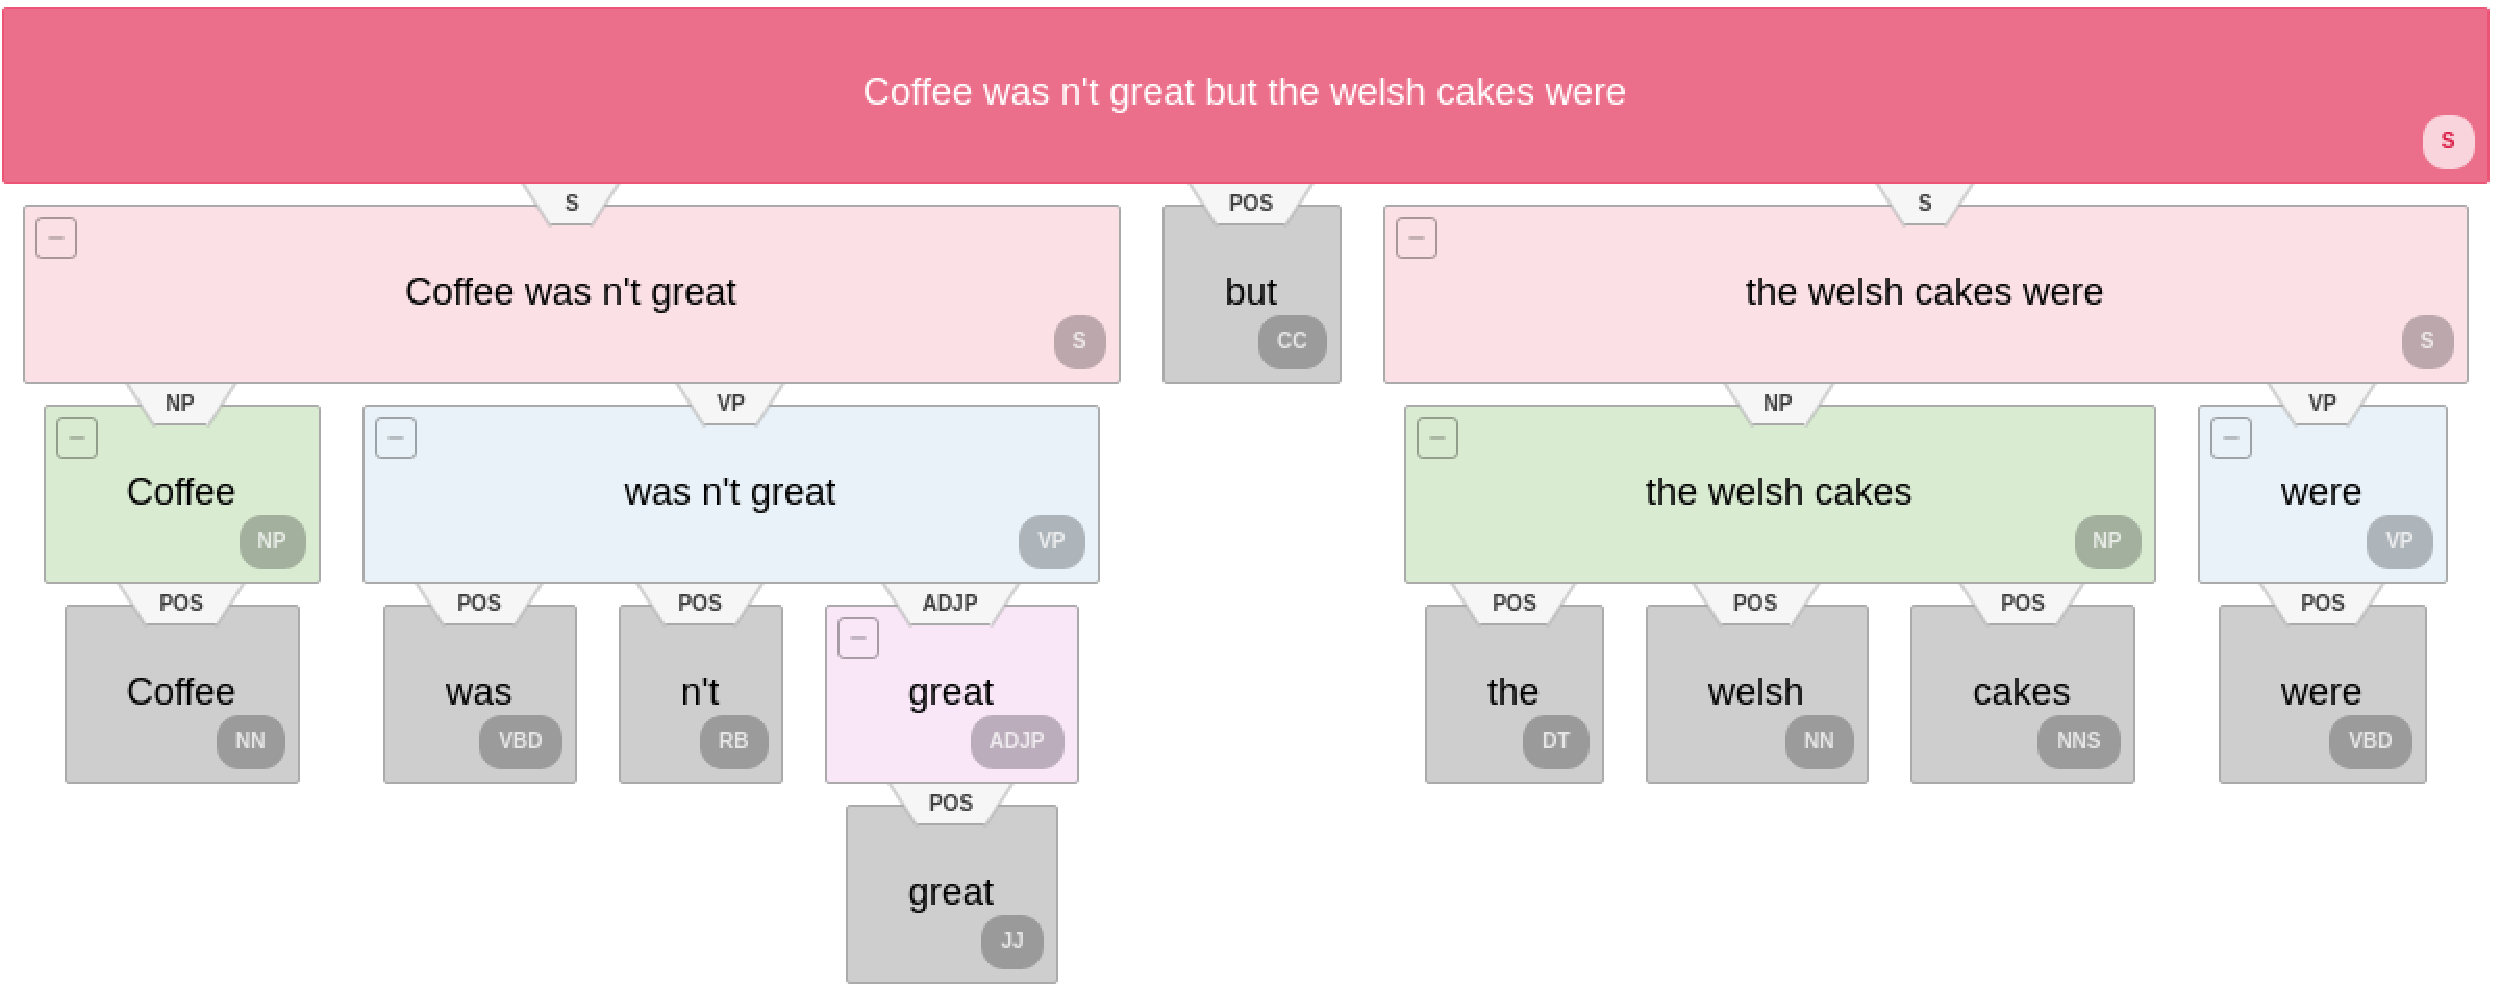
\includegraphics[scale=0.28]{images/lit_review/constituency_tree.pdf}
    \caption{Constituency tree for the sentence `Coffee wasn't great but the welsh cakes were'. The labels in each box represents the constituency label for that span, the labels for the leaf nodes are the POS tags for those words. The tree was created using the AllenNLP demo, which used \citet{joshi-etal-2018-extending} model.}
    \label{fig:lit_review_constituency_tree}
\end{figure}

\begin{figure}[!h]
    \centering
    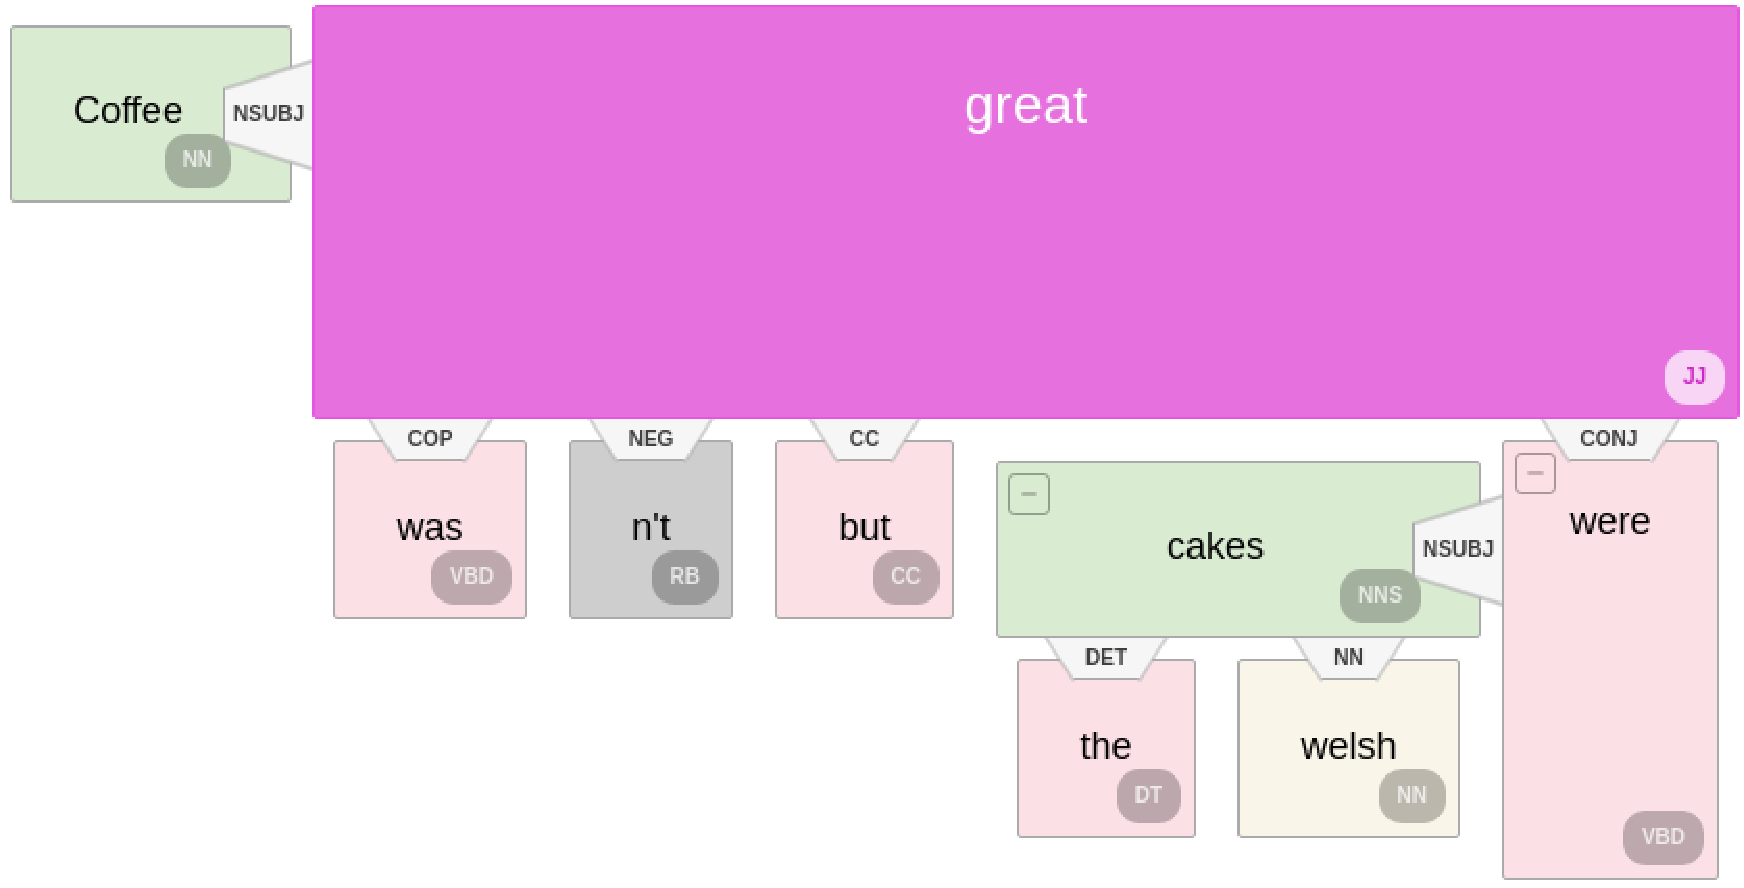
\includegraphics[scale=0.28]{images/lit_review/dependency_parse_tree.pdf}
    \caption{Dependency tree for the sentence `Coffee wasn't great but the welsh cakes were'. The labels within the arcs are dependency labels, and the labels within each box represents the POS tag for the given word. An arc from \textit{word A} to \textit{word B} indicates that \textit{B} is modifying \textit{A}, where \textit{A} is the head word. For example \textit{great} is the head word of \textit{coffee}. The tree was created using the AllenNLP demo, which used \citet{DBLP:conf/iclr/DozatM17} model.}
    \label{fig:lit_review_dependency_parse_tree}
\end{figure}

\section{Sentiment Analysis}
Sentiment analysis can be seen as a more general topic that contains multiple different sub-tasks. These tasks tend to be related and often have different assumptions. In this section, various coarse grained sentiment tasks within sentiment analysis will be discussed starting with the most coarse, document level, and ending with aspect based. During the discussion some important concepts within NLP will also be introduced such as different neural network methods. Throughout the section the different tasks will be shown how they link to each other. The summary of coarse grained sentiment analysis is a primer to the fine grained sentiment analysis review in section \ref{section:lit_review_fine_grained_sentiment_analysis_intro}, which contains the main topic of this thesis Target Dependent Sentiment Analysis (TDSA).

%At the end of the section, the different sentiment tasks will be explicitly shown in terms of how they are related to the main topic of this thesis which is Target Dependent Sentiment Analysis (TDSA).
% Need to mention at the end of this paragraph about poor evaluation and the lack of error analysis showing where alogrthims improve e.g. for generlaising to new targets or targets that exist but with different sentiment. something amybe about generlisation as well.

The many methods that have been used to tackle TDSA and all NLP problems fall into three different categories; supervised, unsupervised, and semi-supervised. Supervised methods require labelled data, in the case of sentiment analysis this would be sentiment labels attached to their relevant text \citep{pang-etal-2002-thumbs}. Unsupervised methods on the other hand only require unlabelled data, which in the sentiment analysis case is just the text. Unsupervised methods within sentiment analysis are normally based around sentiment lexicons (lists\langcorrections{Added s} of words that have an attached sentiment) \citep{hu2004mining} and sometimes a combination\langcorrections{Removed s} of rules \citep{Hutto2014VADERAP}. Thus unsupervised methods tend to require some prior knowledge. Finally,\langcorrections{Added comma} semi-supervised is a combination of the two, learning from both the labelled data and extra unlabelled data \citep{zhu2005semi}. For a more complete overview of the differences between supervised, unsupervised and semi-supervised,\langcorrections{Added comma} see \citet{Weston2007LargeScaleSL}.

\subsection{Document Sentiment Analysis}
The most common sentiment analysis task is that of document level. The task here is given a document which is made up of multiple sentences, to predict the sentiment with the assumption that the document is about one topic \citep{nasukawa2003sentiment}. An example sample for this task can be seen in example \ref{example:lit_review_document_sentiment} where the sentiment of the whole document/review is assumed to be about the movie that is being reviewed. The first to apply a supervised machine learning algorithm to this problem was \citet{pang-etal-2002-thumbs}, where they applied several Machine Learning (ML) classifiers with Bag Of Words (BOW) as features to a new movie review dataset. This line of research of applying ML was further extended by \citet{pang-lee-2004-sentimental} who found that they could reduce the number of sentences by removing objective sentences in the document without significantly impacting, and in some cases improving, the overall accuracy of the classifier. \citet{mullen-collier-2004-sentiment} explored incorporating more semantic features into the BOW models such as the average sentiment values based on the unsupervised techniques of \citet{turney-2002-thumbs}. This approach of adding more semantic information into BOW models was further explored by \citet{whitelaw2005using} who created lexicon feature sets based around appraisal groups. Even though the use of semantic information had improved results \citep{whitelaw2005using}, the strong baseline performance of just using n-gram BOW features was further investigated by \citet{martineau2009delta} who showed that incorporating the class into the TF-IDF weighting mechanism \citep{jones1972statistical} to create Delta TF-IDF significantly improved results. However Delta TF-IDF was only created to work with two classes\footnote{In the sentiment case this is the positive and negative classes.} and not shown to generalise to \textit{n} classes. However a future study by \citet{paltoglou-thelwall-2010-study} showed that further performance gains can be made to TF-IDF based systems by using more enhanced weighting systems like BM25 \citep{robertson1995okapi}.\langcorrections{Indentation added to Example \ref{example:lit_review_document_sentiment}}

\begin{example}
\setlength{\parindent}{17pt}
\indent\textit{a couple of criminals ( mario van peebles and loretta devine ) move into a rich family's house in hopes of conning them out of their jewels . however , someone else steals the jewels before they are able to get to them . writer mario van peebles delivers a clever script with several unexpected plot twists , but director mario van peebles undermines his own high points with haphazard camera work , editing and pacing . it felt as though the film should have been wrapping up at the hour mark , but alas there was still 35 more minutes to go . daniel baldwin ( i can't believe i'm about to type this ) gives the best performance in the film , outshining the other talented members of the cast .}
\caption{Negative document level sentiment example. Document ID \textit{cv435\_24355} taken from \citet{pang-etal-2002-thumbs} sentiment dataset.}
\label{example:lit_review_document_sentiment}
\end{example}

The supervised approaches that have been mentioned so far use a BOW approach, of which this form of vector representation is limited in what it can represent. BOW approaches that use n-gram word features can only learn what a word means within that \textit{n} window. For instance take \textit{n} to be 1 and 2\footnote{i.e. uni-gram and bi-gram features.} it would understand terms such as `very good' and `good' where both would be associated with positive sentiment, however if the statement was `not very good' then it would not capture the full sentiment as it would require all three words to know it is negated. One approach would be to have a very large value for \textit{n}, but this would create a very sparse vector representation which would not generalise well \citep{le2014distributed}. Thus the move away from BOW sparse vector representations to dense word representations was shown to be promising for sentiment analysis in \citet{maas-etal-2011-learning} work. However, this work only found better performance than BOW when they combined the dense vectors with the BOW sparse vector. This first step into dense representation did show some promise as the representation can be learnt from unlabelled data, where they found that results increased when more unlabelled data was used. These dense representations are very similar to what a traditional BOW model learns through its weights within the model \citep{goldberg2017neural}\footnote{See section 2.5.}. The benefit of using the dense representations on the downstream task (sentiment analysis) is that a good representation of the vectors can be learnt from another unsupervised task from unlabelled data first\footnote{The task can also be supervised, but would require labelled data.}. Thus allowing the model to have prior knowledge of what words mean (semantically and syntactically \citep{mikolov2013efficient}) encoded into the vector representation before training the model, unlike the BOW representation which contains no prior knowledge. 

\citet{le2014distributed} showed for the first time how dense vector representations using a NN could surpass BOW representation for which \citet{wang-manning-2012-baselines} set a high baseline at the time for a BOW method. \citet{le2014distributed} created dense document/paragraph vector representations that in comparison to the prior word level versions \citep{maas-etal-2011-learning} could encode document size texts without averaging by learning to predict the next word within a small context window from the document, thus each document vector would be different unlike the word representations\footnote{Unless two or more documents are identical.}. \citet{johnson-zhang-2015-effective} showed that without any additional unlabelled data unlike \citet{le2014distributed} a Convolution NN (CNN) can outperform the BOW approach. The CNN can be seen as a NN approach to a BOW model whereby\langcorrections{Removed space.} the CNN has a set of user defined window sizes of which these window sizes are analogous to n-grams in a BOW model. The CNN differs from the BOW model as it can generalise to unknown n-gram sequences, as it learns how to combine representation from multiple word representations to create the n-gram representation. In comparison for the BOW model it learns what that entire n-gram means and disregards similarities between n-grams based on the words within the n-gram. Furthermore the CNN model does not have the sparsity problem that a BOW model has thus the window size (n-gram in BOW case) can be large;\langcorrections{Added ;} e.g. \citet{johnson-zhang-2015-effective} found that having a window size of 2 and 3 performed\langcorrections{Removed `to` and added `ed` to perform} best\footnote{\citet{le2014distributed} has a good summary of the drawbacks of BOW vector representations.}. For a more complete overview of CNNs, the reader is directed to chapter 13 of \citet{goldberg2017neural}.

None of the above methods, including the NN approach, take into account the word order of the whole document. One family of NN that explicitly encodes the whole sequences\langcorrections{Added `s`} of text in order is the Recurrent NN (RNN) \citep{rumelhart1985learning}. The RNN has several popular variants; Long Short Term Memory (LSTM) \citep{hochreiter1997long} and the Gated Recurrent Unit (GRU) \citep{cho-etal-2014-learning}. \citet{dai2015semi} showed practically that LSTMs can be used for long sequence classification tasks such as document sentiment classification. \citet{xu-etal-2016-cached} created the Cached LSTM to better encode information from large sequences of text, like documents, and showed that it can outperform the LSTM on document sentiment analysis. Hierarchical \citep{zhang2015character} and dilated \citep{strubell-etal-2017-fast} CNN approaches have been created which can capture large contexts,\langcorrections{Added comma} e.g. sentences rather n-grams, where they have been shown to be\langcorrections{added words `to be`} successful in sentiment analysis \citep{conneau-etal-2017-deep}. Finally and more recently, the transformer NN \citep{vaswani2017attention} approach has been applied which does not preserve word order (like the RNN or CNN) but rather treats the text more like a tree structure through attention mechanisms, whereby each word learns to contextualise itself within the text (can be the whole text). The transformer success can be best seen through BERT \citep{devlin-etal-2019-bert} where the architecture can be applied to a task like document sentiment analysis \citep{sun2019fine}\footnote{For a good comparison of RNN, CNN, and transformer based models with respect to computational cost see section 4 of \citet{vaswani2017attention}.}. 

The majority of these more recent NN approaches have been tested on much larger sentiment datasets (100Ks of documents) compared to the earlier work (2-25K documents). It has also been shown that for some of these NN approaches to work well they require extra data \citep{dai2015semi}. However it was found in \citet{dai2015semi} that these NN approaches can make great use of unlabelled data through a language modelling objective. This technique of training on one or more datasets and/or tasks before then applying the model to the end task (in this case document sentiment analysis) is defined as transfer learning in this thesis \citep{ruder2019neural}\footnote{Chapter 3.}.  Both \citet{howard-ruder-2018-universal} and \citet{sun2019fine} found that by pretraining (a type of transfer learning) on the unlabelled data can have large performance gains, making the models more sample efficient with respect to labelled/annotated data. All of the neural methods within this and the last paragraph take into account large contexts of the document,\langcorrections{added comma} if not the whole document, whereas none of the previous methods could effectively do so. This allows the methods to overcome one the main challenges in document sentiment analysis that both \citet{turney-2002-thumbs} and \citet{pang-etal-2002-thumbs} found where the sentiment of the whole document is not the ``sum of the parts'' \citep{turney-2002-thumbs}.

The approaches taken so far treat the document as one large object to encode using some form of supervised method. However there have been methods proposed that suggest it is better to break the document up into smaller linguistic units to encode first into some form of intermediate representation, which is then later combined to generate a sentiment value for the whole document. \citet{bhatia-etal-2015-better} used Rhetorical Structure Theory (RST) \citep{mann-1984-discourse} to create a discourse structure for the document, which\langcorrections{Removed `of` and `this`} can be represented as a dependency-based discourse tree where the nodes are represented by Elementary Discourse Units (EDUs). They found that weighting the outputs of different supervised and unsupervised methods applied to EDUs in the tree based on their depth within the tree improved results. \citet{yang-etal-2016-hierarchical} used sentences to represent the whole document and weighted these sentences and the words within each sentence using two supervised attention mechanisms\langcorrections{Added `s`}. Thus this method unlike \citet{bhatia-etal-2015-better} learnt which sentences and words within those sentences were important to the document's sentiment rather than having a predefined weighting mechanism.

\citet{pang-etal-2002-thumbs} created the first English dataset of movie reviews (1.4K documents), which was later revised and increased in \citet{pang-lee-2004-sentimental} (2K documents), and then increased a lot further by \citet{maas-etal-2011-learning} (25K documents). The prior datasets all contained only two classes, positive and negative, and these were based on the star rating that the movie review was given by the user. \citet{zhang2015character} created four much larger datasets ($600$K -- $4$M\langcorrections{Corrected} documents) that\langcorrections{Removed `have`} originated from Yelp\footnote{https://www.yelp.com/dataset} and Amazon reviews \citep{mcauley2015image} which contain between two and five classes where the classes are based around the user's star rating. This list of English datasets is not supposed to be exhaustive but is given as reference to popular and widely used datasets from the past and current literature.

In this sub-section, document sentiment analysis has been covered with respect to supervised methods and the associated popular English datasets. From the literature it is clear to see that the SOTA are NN based methods that require some form of transfer learning \citep{yang2019xlnet}. All of the methods also clearly point to one of the main challenges in document sentiment analysis which is how best to contextualise the whole document. In the early methods, such as BOW, the methods could only create local contexts through n-grams. This\langcorrections{Added full stop and capitalised `T` on `This`} was\langcorrections{Removed `then`} overcome with NN approaches such as the LSTMs, hierarchical CNNs, and transformers being able to capture the global context of all tokens in the document. Finally within this sub-section different NN approaches have been explained as well as defining the concept of transfer learning.

\subsection{Sentence Sentiment Analysis}
Sentence level sentiment analysis is very similar to document level,\langcorrections{Added level and comma} whereby the only difference is the length of the text to be processed. Due to the length difference, the task is somewhat conceptually easier as a sentence is less likely to have multiple conflicting sentiments, thus the overall sentiment of the sentence is easier to predict. Many different approaches have been used for sentence-based analysis: BOW \citep{wang-manning-2012-baselines}, CNN \citep{kim-2014-convolutional, kalchbrenner-etal-2014-convolutional}, LSTM \citep{brahma2018improved}, and\langcorrections{Added and} BERT \citep{devlin-etal-2019-bert}. However,\langcorrections{Added comma} similar to document level, ``the sentiment of a sentence is not merely the sum of the polarity of the words and phrases found in the text, but rather depends on a number of compositional phenomena that act on\langcorrections{Changed "of" to "on"} indicators of polarity'' \citep{barnes2019improving}. This problem can be best seen in figure \ref{fig:lit_review_sentence_sentiment_example}\footnote{The sentence was chosen from \citet{barnes2019improving} and the figure was generated using the live demo found at this URL \url{http://nlp.stanford.edu:8080/sentiment/rntnDemo.html}.}, where\langcorrections{Removed by from whereby} it can be seen that even though the sentence has multiple positive words the sentiment of the sentence is dominated by the scope of the negation. Due to this, many approaches have been taken to better model the sentiment phrases within the sentence using BOW with compositional semantics \citep{choi-cardie-2008-learning}, Conditional Random Field (CRF) \citep{nakagawa-etal-2010-dependency}, Recursive NN (RCNN) \citep{socher-etal-2012-semantic},\langcorrections{Added comma} deep RCNN \citep{irsoy2014deep}, Tree-LSTM \citep{tai-etal-2015-improved}, Graph NN (GNN) \citep{zhang-zhang-2019-tree}, and multi task learning whereby negation scope and cue detection are the auxiliary task \citep{barnes2019improving}.\langcorrections{In \ref{fig:lit_review_sentence_sentiment_example} complete, removed the `by` after the word `where`.}

\begin{figure}[!h]
    \centering
    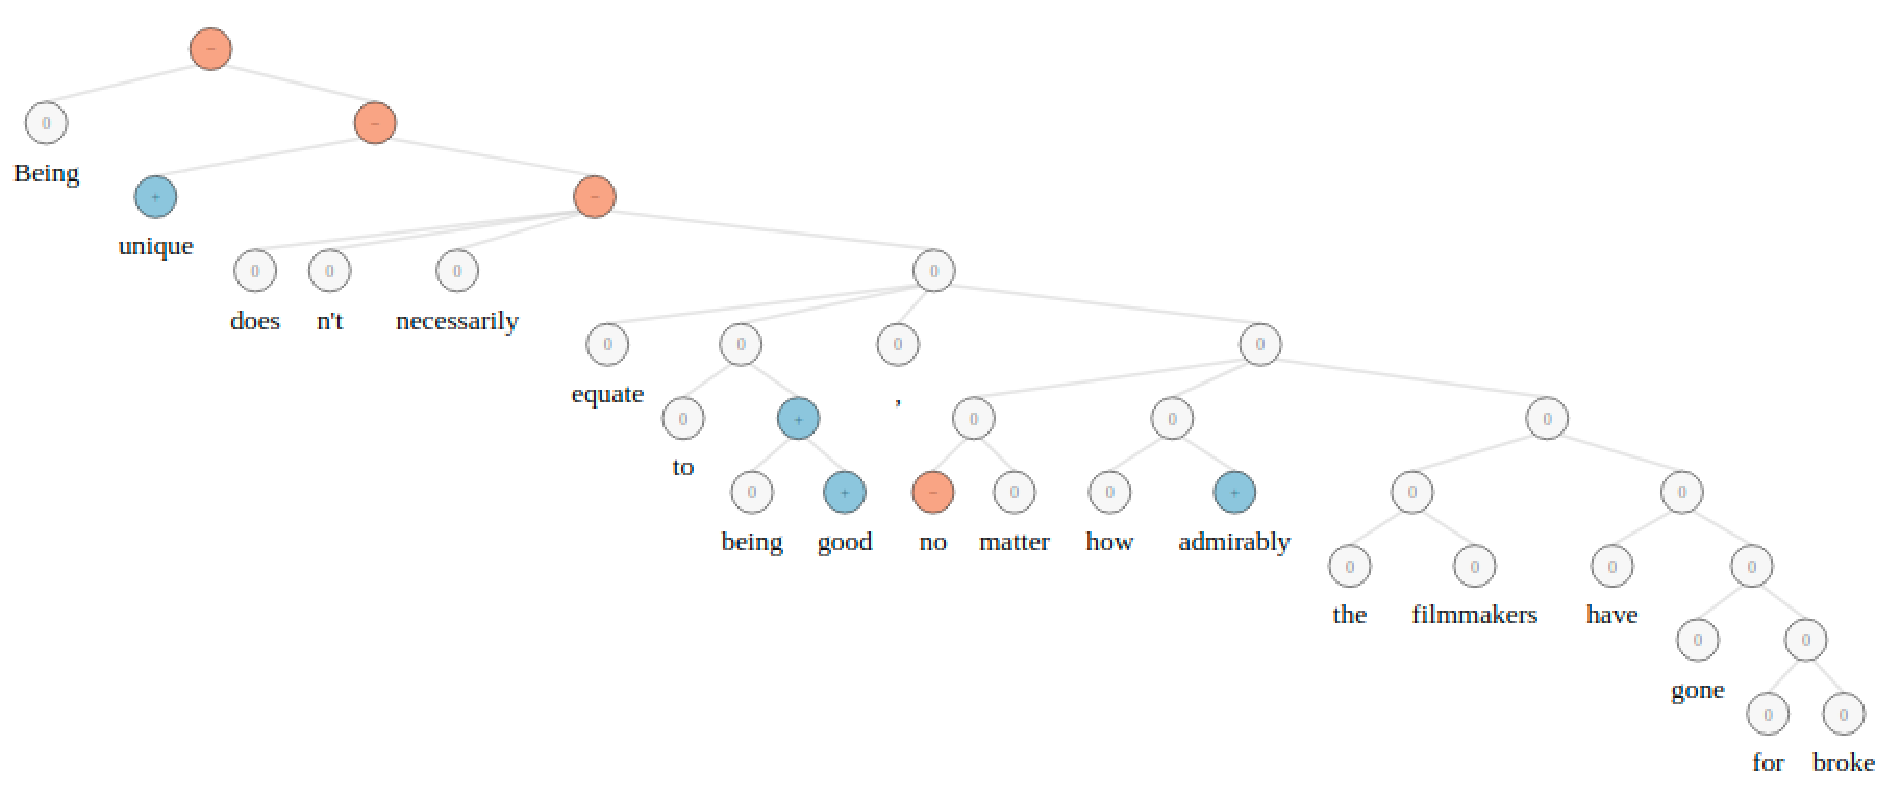
\includegraphics[scale=0.35]{images/lit_review/sentence_sentiment_example.pdf}
    \caption{Phrase and overall sentiment from~\citet{socher-etal-2013-recursive} model, where red, white, and blue represent negative, neutral, and positive sentiment respectively. The sentence in the figure is `Being unique doesn’t necessarily equate to being good, no matter how admirably the filmmakers have gone for broke'.}
    \label{fig:lit_review_sentence_sentiment_example}
\end{figure}

\citet{socher-etal-2013-recursive} took modelling phrases within sentences further by creating a dataset where\langcorrections{Removed "by"} each phrase from the \citet{pang-lee-2005-seeing} movie dataset was manually annotated with a sentiment value, which\langcorrections{Removed "of" and "this"} can be seen in figure \ref{fig:lit_review_sentence_sentiment_example} whereby the model output shown is how the dataset is annotated. Thus this dataset allows models to better capture the compositional phenomena more explicitly by using the phrase level annotation. In a similar trend,\langcorrections{Added comma} \citet{yang-cardie-2014-context} found\langcorrections{Removed "that"} using inter- and intra-sentence\langcorrections{Added hyphens} discourse features to be useful,\langcorrections{Added comma} showing that sentence level classification can be dependent on surrounding sentences. Similarly \citet{mcdonald-etal-2007-structured} found that jointly modelling the sentence and document classification tasks helps improve both. More recently,\langcorrections{Added comma} \citet{angelidis-lapata-2018-multiple} found that by framing document classification as a multiple instance learning (MIL) \citep{dietterich1997solving} problem they were able to create a sentence (EDU) classifier using only the document labels, this outperformed a fully supervised sentence (EDU) level classifier. This MIL method was also shown to be useful when applied to the food health domain \citep{karamanolakis-etal-2019-weakly}.

This review has shown that sentence level sentiment requires both understanding the complex structure within the sentence as well as the more global content of the document. However, even though the literature shows the use of explicitly taking into account phrases and document level information,\langcorrections{Added comma} current SOTA uses the same techniques as that of document level \citep{yang2019xlnet}, utilising transfer learning mainly from a language modelling task. Even so,\langcorrections{Added comma} \citet{barnes-etal-2019-sentiment} have\langcorrections{Changed "has" to "have"} annotated the errors coming from SOTA models into eighteen different categories finding that they perform badly on sentences containing non-standard spellings, idioms, and world knowledge,\langcorrections{Added comma} to name a few. This shows that sentence level sentiment analysis still has plenty of error cases to solve through better incorporating linguistic and world knowledge into new and/or existing methods. To clarify,\langcorrections{Added comma} all of the research mentioned on sentence level sentiment analysis was applied and thus to some extent developed for English. 

\subsection{Aspect Based Sentiment Analysis}
Document and sentence level sentiment analysis both assume that they are discussing one topic \citep{liu2015sentiment}\footnote{Page 47-48.}, for instance if the document (sentence) comes from a review (headline of a review) of the movie, \textit{The Avengers}, the topic that the sentiment is assumed to be about is the movie, \textit{The Avengers}. However, both documents and sentences can contain sentiments on multiple different topics not just the main overall topic of the entire review. Aspect Based Sentiment Analysis (ABSA) attempts to overcome this problem, instead of predicting one sentiment for a document or a sentence it predicts multiple sentiments conditioned on multiple different predefined aspects/topics. ABSA can be performed at different linguistic granularities,\langcorrections{Added comma} typically either document or sentence level. Example \ref{example:lit_review_document_aspect_sentiment} is a Tripadvisor review taken from \citet{Wang2010LatentAR} with seven aspects and their respective sentiments\footnote{They were actually ratings rather than sentiments, but the ratings are used as approximations for sentiment.}, as well as the overall sentiment of the hotel. From this document level ABSA example it can be seen that these aspects are latent, that is the aspect itself does not necessarily occur in the text, this is shown in example \ref{example:lit_review_document_aspect_sentiment} where\langcorrections{Removed "by"} the \textit{service} is negative as the ``Hotel staff speak zero English... The process at the hotel is a bit confusing... staff weren't overly friendly.''. This example would be typically used as a training example for document level ABSA. In this subsection document and sentence level ABSA will be described along with advances in each area and popular datasets.


%Further this example demonstrates that even though the overall sentiment can be negative other aspects can be positive, like the \textit{value} of the hotel. Thus illustrating why document and sentence level sentiment analysis is too coarse and why a more fine grained approach like ABSA is required. 

\begin{example}
\textit{Good and clean but no English spoken The good: The hotel is in a great location and withing walking distance to the Forbidden City and some other sights in this hisrotic district. The rooms were comfortable and clean, really good value.The bad: Hotel staff speak zero English. Breakfast is only Chinese breakfast. The process at the hotel is a bit confusing (make sure you keep those pink receipts they give when you pay, you need them to check out!) and staff weren't overly friendly. Internet is expensive and slow.}
\caption{Example of document level aspect sentiment analysis. The aspects and their receptive sentiments are: \textit{service} (1), \textit{business service} (2), \textit{cleanliness} (3), \textit{check in / front desk} (2), \textit{value} (4), \textit{rooms} (3), and \textit{location} (4). The sentiments were on a scale of 1-5 and the overall sentiment for the review was 2. This was taken from review id \textit{447367} from the trip advisor review dataset of \citet{Wang2010LatentAR}.}
\label{example:lit_review_document_aspect_sentiment}
\end{example}

\subsubsection{Document-level ABSA}
\label{lit_review_document_ABSA}

\citet{snyder-barzilay-2007-multiple} treated the task of document ABSA as a supervised ranking problem, where each aspect is ranked based on a BOW feature vector. They showed the benefit of modelling dependencies between aspects. They found that 38\% of their restaurant review training data contained the same sentiment for all aspects in their respective reviews. Thus they added an agreement function within their model which predicts whether or not all aspects for the review should contain the same sentiment which significantly improved performance. In comparison \citet{Wang2010LatentAR} created the Latent Rating Regression model, which instead of learning from the aspect sentiments can train the model just from the overall sentiment. This therefore reduces the requirement of more fine grained sentiment training data, but the model did require a set of seed words that represented the aspects e.g. for the aspect \textit{room} a set of key words would be \textit{room}, \textit{suite}, \textit{view}, and \textit{bed}. 

More recently, supervised Neural Network (NN) approaches have been the most popular and successful approach to document ABSA. The first to use a NN for document ABSA was~\citet{lei-etal-2016-rationalizing}, whose main aim was to create rationals/explanations for the predictions given only the aspect sentiment labels for supervision.~\citet{yin-etal-2017-document} showed the importance of biasing the attention mechanism within a hierarchical NN~\citep{yang-etal-2016-hierarchical} towards the aspect of interest. The attention mechanism used a set of keywords to define each aspect, from these keywords the attention mechanism would use a memory network~\citep{weston2014memory} to learn how to best describe the aspect so that the model focused on the most important words and sentences in the document.~\citet{yin-etal-2017-document} benchmarked their approach across numerous neural and non-neural approaches.~\citet{li-etal-2018-document} used a similar hierarchical NN as~\citet{yin-etal-2017-document} and found significant performance gains when incorporating both user\footnote{On the dataset that contained user information.} and/or the overall document sentiment information into the attention network. They found that the document sentiment information is useful as the related aspect sentiments are correlated. Further the user information allows the model to better capture textual and sentiment similarities at the aspect level, e.g.,\langcorrections{Added commas} a user tends to have similar sentiment scores for aspects across documents and tends to describe aspects in a similar manner across documents. Finally, the most recent and successful approach used a hierarchical neural Reinforcement Learning (RL)~\citep{williams1992simple} method~\citep{wang-etal-2019-human}\footnote{They called document ABSA, Document-level Aspect Sentiment Classification (DASC).}, whereby\langcorrections{Removed space between "where" and "by"} instead of splitting the document into sentences they used Elementary Discourse Units (EDUs). They used the RL approach to first find aspect relevant EDUs and then within the EDU the relevant aspect sentiment words. They found that if they had used sentences instead of EDUs\footnote{They call EDUs clauses.} then the performance would have decreased by 2.44\% on average, of which they believe this is due to 90\% of EDUs only containing one sentiment~\citep{bayoudhi2015sentiment}. Through error analysis they found that their method performed poorly when negation is used or a comparison is made, however they did not quantify the number of times these errors where made.
% I think we should talk here about sentence level ABSA as the AE literature evaluates some what on both.

% There is also the SemEval review level datasets
There are three main datasets to evaluate document ABSA, Tripadvisor \citep{Wang2010LatentAR}\footnote{This is sometimes called TripDMS.}, BeerAdvocate \citep{mcauley2012learning}, and TripUser \citep{li-etal-2018-document}. Both the Tripadvisor and BeerAdvocate datasets since have been reprocessed by \citet{yin-etal-2017-document} so that aspect sentiments per document are less correlated\footnote{The standard train, development, and test splits for the Tripadvisor and BeerAdvocate datasets can be found here \url{https://github.com/HKUST-KnowComp/DMSC}.}\footnote{The less correlated method comes from \citet[\S5.1]{lei-etal-2016-rationalizing}. They train a linear regression model to predict one of the aspect's sentiment based on all the other aspects sentiments, they then pick the documents that have the largest error until the aspect sentiment correlation in the documents goes beyond a certain threshold.}. This technique of reducing the correlation of the aspect sentiments per document was suggested by \citet{lei-etal-2016-rationalizing}, to ensure that the model does not get ``confused''. It has not been shown whether training models on datasets that have less correlation between aspect sentiments per document produce better models, further \citet{snyder-barzilay-2007-multiple} actually exploited this correlation in their modelling. The Tripadvisor and TripUser are both hotel reviews from the Tripadvisor website\footnote{\url{https://www.tripadvisor.co.uk/}} and contain the same seven aspects, but the TripUser dataset also contains user information unlike Tripadvisor. The BeerAdvocate dataset comes from a beer review website Beeradvocate\footnote{\url{https://www.beeradvocate.com/}} and contains four aspects.

% Need to talk about some point the use of document level as a summary of sentence level which is useful for review websites.
The datasets mentioned so far are all the datasets that have been used\footnote{Or derivatives of.} in the prior work stated in this thesis so far. However these datasets are not expertly annotated data, rather the data has been scraped from their representative websites where the reviews were `annotated' by many different users. One of the few datasets that has been annotated by experts is the SemEval 2016 task 5 subtask 2 dataset~\citep{pontiki-etal-2016-semeval}, which contains seven datasets in five different languages and varies\langcorrections{changed "vary" to "varies"} across three domains\footnote{Restaurant, laptop, and hotel reviews.}. The only methods that have been applied to these datasets are those that entered the SemEval competition.

\subsubsection{Sentence ABSA}
\label{lit_review_sentence_ABSA}

Sentence ABSA unlike document ABSA tends to contain far fewer aspects within its text and unlike document it is rare for a sentence to have all aspects, which is not the case in document ABSA \citep{snyder-barzilay-2007-multiple, Wang2010LatentAR}. All document ABSA methods could be applied to sentence ABSA with minimal changes, however the vast majority of them have been designed for longer texts, for instance the hierarchical NN methods \citep{yin-etal-2017-document, li-etal-2018-document, wang-etal-2019-human}. To further iterate this point on a sentence containing few aspects per sentence,\langcorrections{Added comma} examples \ref{example:lit_review_sentence_aspect_sentiment_1} and \ref{example:lit_review_sentence_aspect_sentiment_2} show two different sentences from the widely used SemEval 2014 task 4 subtask 4 restaurant review dataset \citep{pontiki-etal-2014-semeval}, containing\langcorrections{Removed "each"} one and two aspects respectively. Further,\langcorrections{Added comma} the statistics from the SemEval 2014 restaurant training dataset state that on average each sentence will only have 1.22 aspects\footnote{This was calculated based on the training datasets containing 3041 sentences of which in total there are 3713 aspects within that dataset.} \citep{pontiki-etal-2014-semeval}. In comparison to document, sentence ABSA is less likely to have an \textit{overall} sentiment\footnote{\textit{Overall} sentiment here refers to sentence or document level sentiment, rather than an \textit{overall/general} aspect sentiment e.g. the aspect \textit{RESTAURANT\#GENERAL} in the SemEval 2015 task 12 restaurant dataset \citep{pontiki-etal-2015-semeval}.}, of which some document approaches have made use \langcorrections{removed "of this"}\citep{Wang2010LatentAR, li-etal-2018-document}. Lastly,\langcorrections{Added comma} document ABSA in effect\langcorrections{Changed "affect" to "effect"} summarises the sentiment information for each aspect that has been captured throughout the document, which can make document sentiment analysis a more difficult task if there are lots of contradicting sentiments\langcorrections{Added "s"} for one aspect \citep{pontiki-etal-2016-semeval}.  


\begin{example}
\textit{Overall I would recommend it and go back again.}
\caption{Example of sentence level aspect sentiment analysis. Contains one aspect \textit{anecdotes/miscellaneous} with positive sentiment. This was taken from sentence id \textit{2609} from the trail restaurant dataset of \citet{pontiki-etal-2014-semeval}.}
\label{example:lit_review_sentence_aspect_sentiment_1}
\end{example}

\begin{example}
\textit{Even though its good seafood, the prices are too high.}
\caption{Example of sentence level aspect sentiment analysis. Contains two aspects \textit{food} and \textit{price} with positive and negative sentiment respectively. This was taken from sentence id \textit{3440} from the trail restaurant dataset of \citet{pontiki-etal-2014-semeval}.}
\label{example:lit_review_sentence_aspect_sentiment_2}
\end{example}

Sentence ABSA was popularised by task 4 in SemEval 2014 \citep{pontiki-etal-2014-semeval} where 20 teams created various methods. The winner,\langcorrections{Added comma} \citet{kiritchenko-etal-2014-nrc},\langcorrections{Added comma} used a Support Vector Machine (SVM) \citep{chang2011libsvm} with different BOW features including ngrams, POS tags, and various in and out of domain sentiment lexicon features\footnote{Sentiment lexicon is a collection of different groups of words where each group is associated to a specific sentiment. This definition follows that of \citet{mohammad-turney-2010-emotions} for their emotion lexicon definition if you substitute emotion for sentiment.}. To\langcorrections{Removed "Further"} better capture the aspect specific sentiment,\langcorrections{Added comma} they utilised a domain adaptation technique \citep{daume-iii-2007-frustratingly} such that each aspect category had its own BOW weight vector that was learnt at the same time as the general BOW weight vector, so that aspect specific and general features can be learnt separately. SemEval repeated a similar task for two more years, 2015 and 2016, where\langcorrections{replaced "when" with "where"} the winners all use a similar BOW approach \citep{saias-2015-sentiue, brun-etal-2016-xrce, kumar-etal-2016-iit}. 

NN approaches for this task are desirable due to them requiring fewer linguistic resources, and the ease of transferring the approach to multiple languages \citep{ruder-etal-2016-insight-1}. \citet{ruder-etal-2016-insight-1} applied a CNN to the task outperforming many of the aforementioned BOW approaches on multiple languages. In later work \citet{ruder-etal-2016-hierarchical} showed that taking into account the surrounding sentences using an hierarchical LSTM further improved results. \citet{wang-etal-2016-attention} found that by adding attention to a sentence level LSTM improved the model by allowing it to better capture relevant aspect specific words within the sentence. Follow on work \citep{bao-etal-2019-attention} found that regularising the attention network using sentiment lexicons and/or attention sparsity improved the robustness of the model. \citet{wang2018aspect} utilised a hierarchical NN similar to \citet{yin-etal-2017-document} (document ABSA) whereby the hierarchy of the sentence was based around EDUs within the sentence, and the words within those EDUs. This was proposed on the premise that EDUs often discuss one aspect, thus making the task for the NN easier, as the model could ignore EDUs that were not discussing the relevant aspect. They found this hierarchical approach to outperform the flattened version. Current SOTA approaches utilise transfer learning from Bi-directional Language Models (BiLM) \citep{sun-etal-2019-utilizing, jiang-etal-2019-challenge} (also known as Contextualised Word Representations (CWR) which is what they will be called from now on).\langcorrections{Explained CWR}

Compared to the previous approaches \citet{kaljahi-foster-2018-sentiment} explored whether adding the aspect's sentiment expressions to a model would improve results. The sentiment expression which is ``part of the sentence which conveys the sentiment towards a certain aspect'' \citep{kaljahi-foster-2018-sentiment} was added to the English SemEval 2016 laptop and restaurant datasets. Example \ref{example:lit_review_sentence_aspect_sentiment_expression} demonstrates what an aspect's\langcorrections{added apostrophe} sentiment expression is. They found that\langcorrections{Replaced "by" with "that"} adding the sentiment expressions into the NN model improved results greatly, however in this setup at test/inference time the model would require the aspect's\langcorrections{Added apostrophe} sentiment expression. To overcome this they incorporated the sentiment expressions in a multi task setup, but this led to the model performing as well as a model that did not require sentiment expressions. This line of research shows promise as it demonstrates that using aspect sentiment expressions can improve results but incorporating this information into a model that does not require it at test time is difficult. Further aspect sentiment expressions, if they could be predicted at the same time as the sentiment, could create some form of explanation to the sentiment prediction, making the black box NN methods more explainable,\langcorrections{Added comma} which is similar to what \citet{lei-etal-2016-rationalizing} did in document ABSA.

\begin{example}
\textit{However, go for the ambience, and \textbf{consider the food just a companion} for a trip across the world!}
\caption{Aspect sentiment expression example, where the sentiment expression is in \textbf{bold} for the related aspect \textbf{food\#quality}. This was taken from the SemEval 2016 Restaurant dataset \citep{pontiki-etal-2016-semeval} with the additional sentiment expression labelled by \citet{kaljahi-foster-2018-sentiment}.}
\label{example:lit_review_sentence_aspect_sentiment_expression}
\end{example}

% Need to mention at some point the link between the 2016 sentence and document ABSA this is not the same as target also linked through the sentence and i assume review id.
Popular sentence ABSA datasets for English are the SemEval 2014\footnote{The restaurant ABSA dataset partially came from \citet{Ganu2009BeyondTS}.} \citep{pontiki-etal-2014-semeval}, 2015 \citep{pontiki-etal-2015-semeval}, and 2016 \citep{pontiki-etal-2016-semeval} datasets for the laptop, restaurant, and\langcorrections{Added "and"} hotel review domain\footnote{The 2014 datasets ABSA annotation was only provided for the restaurant domain.}. A large difference between the 2015 and 2016 datasets compared to the 2014 was the sentiment of an aspect may require a larger context than just the sentence the aspect appeared in, hence why the whole review was given as context. The 2016 SemEval dataset also expanded the number of languages from just English to six more languages\footnote{The six languages are; Dutch, French, Russian, Spanish, Arabic, and Chinese.}. Also,\langcorrections{Added comma} as stated in the last paragraph, \citet{kaljahi-foster-2018-sentiment} annotated the English SemEval 2016 laptop and restaurant dataset with sentiment expressions. There has also been a challenge dataset, Multi-Aspect Multi-Sentiment (MAMS) \citep{jiang-etal-2019-challenge}, which is within the restaurant review domain\footnote{This dataset was created from the same source of restaurant reviews as the SemEval 2014, 2015, and 2016 restaurant dataset, which was the Citysearch New York dataset by \citet{Ganu2009BeyondTS}.}, unlike the other datasets it ensures that each sentence contains at least two aspects and at least two different sentiments per sentence.

Sentence level ABSA has also been known as topic sentiment analysis within the Twitter sentiment analysis community. Topic sentiment analysis has been run as a competition three times at SemEval \citep{rosenthal-etal-2015-semeval, nakov-etal-2016-semeval, rosenthal-etal-2017-semeval}, each year creating a new larger dataset for English and in the final year (2017) creating an Arabic Twitter dataset as well. In their first year of running the competition (2015) they also ran a task (D) which they described as ``sentiment towards a topic in a set of tweets'' which can be viewed as a document ABSA task. These datasets are also annotated for Tweet/sentence sentiment as well as the topic, the 2017 dataset contains user information, and the 2015 dataset is also annotated with sentiment expressions.

From this section on ABSA prior work it is clear that there is plenty of future work that can be explored. Creating more robust models is important,\langcorrections{Added comma} especially for real world applications.\langcorrections{Added "s" and removed "of which"} \citet{bao-etal-2019-attention} explored this problem, however they only evaluated on one dataset, thus expanding this evaluation for more datasets and across a spectrum of low to high resource settings would be of use to better understand how robust their method is. An unexplored area is the link between sentence and document ABSA whereby one would assume that document ABSA should improve the performance of sentence and vice versa, of which this can be empirically tested using the SemEval 2015 \citep{pontiki-etal-2015-semeval} and 2016 \citep{pontiki-etal-2016-semeval} review datasets.



% For a good overview of cross-lingual approaches to sentiment analysis at both the sentence and target level see \citet{barnes2019cross} thesis.

%\citet{marcheggiani2014hierarchical} used a CRF model with various BOW features for aspect identification and sentiment prediction, where by they found jointly modelling the aspect and overall review sentiment to be beneficial for aspect sentiment prediction but not identification. Further they also introduced a sentence level English ABSA dataset with review/document level annotation for the hotel domain. 
%Adding user information into sentiment analysis methods has been done

%In a similar line of work Aspect Extraction (AE) is the task of predicting the aspects that the text is discussing, again AE can also be performed typically at document or sentence level. In example \ref{example:lit_review_document_aspect_sentiment} the review has a set of predefined aspects, but not all reviews will always have all of these predefined aspect some may have fewer aspects, and in other domain like Laptop reviews may contain more aspects. For document AE \citet{titov2008modeling} created Multi-grain LDA (MG-LDA) a modified version of Latent Dirichlet Allocation (LDA) for the task of unsupervised document AE. MG-LDA compared to LDA creates two groups local and global where by they found that a local groups better correspond to aspects. To empirically validate their method they showed that adding the MG-LDA features to the \citet{snyder-barzilay-2007-multiple} model improved results and also out performed using the LDA features instead. The drawback of topic modelling methods like LDA or MG-LDA is the requirement of setting the number of topics that the model is required to generate, and then having to manually label which topics correspond to which aspects, if the topics do correspond to any of the predefined aspects. In comparison to this completely unsupervised approach \citet{mukherjee-liu-2012-aspect} used a set of seed words and known number of aspects/topics to constrain their topic modelling based method, which is similar to \citet{Wang2010LatentAR}. 

% A problem with all of these topic modelling based approaches is that it cannot assign a document/text to an aspect or a number of aspects without, the most interesting part of these type of clustering is that it can define what words are in what aspect clusters.
% The existing models that do use seeds can also generate more topics that have not been seeded and they judge if the topic is relevant by looking at the terms in the topic and judging using human knowledge.

%More recent approaches have moved away from topic modelling like LDA to Neural Networks (NN). \citet{he-etal-2017-unsupervised} used an autoencoder styled unsupervised learning objective where by the NN was trained to reconstruct the encoded sentence from a dense matrix that would represent aspects. From this aspect matrix they could find words associated to an aspect using a similarity function between the aspect matrix and a word's vector representation/embedding. Further they could also assign a text to a single aspect label\footnote{The method could not assign more than one label to a text. This could be done but would require some form of threshold/confidence level on the output of the softmax in equation 6.} based on the output of the NN. This approach was later improved upon by \citet{angelidis-lapata-2018-summarizing} where the aspect matrix was initialised using a weighting approach from the embeddings of known aspect seed words, these seed words and their weighting did come from a limited amount of labelled data. Further they showed the benefit of using a multi task learning objective where by predicting the domain of the sentence\footnote{In this work instead of sentences they used EDUs.} was beneficial, as they believed domain relevant words were also relevant to the aspect. 

%\citet{karamanolakis-etal-2019-leveraging} showed how to better utilise known aspect seed words through a student-teacher distillation model \citep{bucilua2006model, hinton2015distilling}, where by the teacher predicted the probability of each aspect for a sentence based on the frequency of the aspect seed words in the sentence\footnote{A special version of a BOW model.}. The student model then learnt off the teacher's model predictions thus not requiring any human annotated data. The teacher's model was then updated using the student predictions on the training data in a co-training setup \citep{blum1998combining}. Thus allowing the teacher to learn weights for each of the seed words, this improved teacher model then re-taught the student model, of which this process is then repeated until the predictions from the teacher and student are similar. The student model is then used to predict which aspect occurs in the text. The advantage of this student model approach unlike the previous NN approaches \citep{he-etal-2017-unsupervised, angelidis-lapata-2018-summarizing} it allows the student model to be any type of model. However they found that averaging word vectors similar to \citet{he-etal-2017-unsupervised, angelidis-lapata-2018-summarizing} to perform well and outperforms all existing unsupervised approaches\footnote{Approaches that use seed words tend to be called weakly supervised rather than unsupervised. This is due to the approach requiring some knowledge that has had to come from a human annotator. However in this part of the literature review we have grouped the unsupervised and weakly supervised together and have explicitly stated at each point if the method required seed words.}.
% next prehaps talk about different ways these are evaluated, may need to introduce the sentence level stuff.

%In all of the previous work ABSA and AE has been discussed at the document level. However there are some noticeable problems with performing at this granularity. For AE, if the set of predefined aspects is known, like the seven aspects in example \ref{example:lit_review_document_aspect_sentiment}, then in most cases due to the size of the documents most of the aspects will be within the document thus making the task 

%To overcome the problem that aspects can have multiple sentiments throughout a document or a sentence \citet{lazaridou-etal-2013-bayesian} setup the AE and ABSA task at the Elementary Discourse Unit (EDU). They also performed their analysis at this linguistic unit as they hypothesised that either the aspect and/or sentiment that the unit will be discussing will change at the start of an EDU. They found that incorporating knowledge of this aspect/sentiment change into their weakly supervised LDA model for AE and ABSA improved results. However performing AE and/or ABSA at EDU level never progressed any further than this line of work.

%A sample of sentence and Tweet can be seen in example. The reason for grouping both sentence and Twitter based methods is due to the fact that Tweet based methods can be seen as a adaptation of sentence based method to a different type of text. 


%The main difficulty in document sentiment analysis has been shown through it's length Further sentiment lexicons have been defined and numerous NN methods have been introduced. 

%So far the supervised methods within document sentiment analysis have been covered, from which it is clear to see that the SOTA are NN based and require some form of transfer learning \citep{yang2019xlnet}. All of the methods also clearly point to one of the main challenges in document sentiment analysis is the size of the documents. This can be seen from early in the literature where  \citet{turney-2002-thumbs} state that the sentiment of the whole document is not the `sum of the parts'. This therefore means that the whole document needs to be understood in context to fully understand the sentiment which has been shown not possible with the BOW methods. Thus the move to NN approaches such as the LSTMs, heirahcical CNNs, and transformers to overcome this problem.


%can be used to c encode some form of word order within 
%The use of dense vector representations stayed at the forefront to State Of The Art (SOTA) document sentiment classification. 

% created a much large movie review sentiment dataset \citet{maas-etal-2011-learning}
%who explored different information retrieval weighting mechanisms

%\citet{whitelaw2005using} Created a apprisal lexicon through using a list of words that were known to be part of the lexicon as `seed words' and then expanding that list through collocations, WordNet, and thesauri

%Incorporating 

%The first document sentiment dataset was by \citet{pang-etal-2002-thumbs}, which was then later enlarged by \citet{pang-lee-2004-sentimental}

%This novel Machine Learning (ML) work was conducted at the same time as \citet{turney-2002-thumbs} who applied an un-supervised approach to the same problem, both came across the same problem, which is that the sentiment of the review cannot be determined through `sum of it's parts' \citep{turney-2002-thumbs}\footnote{This is paraphrased for grammatical reasons, the actual quote is `sum of the parts'}. This problem is due to both works only using BOW (up to bi-grams) features within their methods, thus their features only take into account local context and limited linguistic knowledge (POS tags in \citet{turney-2002-thumbs}). This problem to some extent started to be alievated with the raise of more 

\section{Fine Grained Sentiment Analysis}
\label{section:lit_review_fine_grained_sentiment_analysis_intro}

Compared to the previous sections, this as the name suggests, is the most detailed granularity of sentiment analysis. Fine grained sentiment analysis is made up of many different tasks where the results of these tasks when combined creates the information required to fully understand a sentiment in context. The literature has been very clear on the following tasks being at the core of understanding sentiment in context \citep{wiebe-1994-tracking, kim-hovy-2004-determining, ding2008holistic, liu2015sentiment}:
\begin{enumerate}
    \item Identifying the holder of the sentiment.
    \item Identifying the target/object of the sentiment within the text\footnote{In \citet{ding2008holistic} they use the word feature to mean target. In \citet{kim-hovy-2004-determining} they use topic to mean target.}.
    \item The sentiment of the holder towards the target.
\end{enumerate}

The information from these three tasks creates a triplet of information (sentiment holder, target, sentiment) to define the whole fine grained sentiment task. To better understand this,\langcorrections{Added comma} example \ref{example:lit_review_fine_grained_sentiment_analysis_1}\footnote{In all examples the target will be in bold, the sentiment words within the text in the colour of their sentiment, and the holder underlined. The sentiment colours are \negbox{pink for negative}, \neubox{grey for neutral}, and \posbox{blue for positive}.} contains five triplets; (author, food, negative), (Jonathan, bara brith, positive), (He, leeks, neutral), (June, Welsh fruit cake, negative), and (June, chocolate cake, positive). 


\begin{example}
\textit{(1) The \textbf{food} at the store was \negbox{horrible}, but \underline{Jonathan} thought the \textbf{bara brith} was \posbox{fantastic}.(2) \underline{He} did think the \textbf{leeks} were \neubox{so so}. However \underline{June} found the \textbf{Welsh fruit cake} to be \negbox{tasteless} but the \textbf{chocolate cake} to be \posbox{great}.}
\caption{Made up fine grained sentiment analysis example written on the 24\textsuperscript{th} May. For reference bara brith is a kind of fruit cake that was created in Wales.}
\label{example:lit_review_fine_grained_sentiment_analysis_1}
\end{example}

The triplet of information, which to some degree, was first defined within \citet{wiebe-1994-tracking} when stating the components of a private state\footnote{Page number 235 of \citet{wiebe-1994-tracking}, defines experiencer, attitude, and object as the components of a private state. Experiencer, attitude, and object can be mapped to holder, target, and sentiment within the triplet of information definition.} has been expanded by \citet{liu2015sentiment} who has created the clearest and most detailed definition so far and builds upon the previous work \citep{wiebe-1994-tracking, kim-hovy-2004-determining, ding2008holistic}. Liu's \citep{liu2015sentiment}\langcorrections{Added apostrophe} basic quadruple definition\footnote{Definition 2.1 in \citet{liu2015sentiment}.} is the same as the triplet so far with the added information of time. The importance of time within the definition is argued as sentiment can change over time, which is of importance for real world applications as one may want to know how a holder's\footnote{A more concrete example of a holder could be a politician, whereby the application may want to see when/if they changed their sentiment towards a bill/law.} sentiment changes. 

This quadruple definition is then expanded to a more detailed quintuple definition\footnote{Definition 2.7 \citet{liu2015sentiment}.}, with the target of the sentiment replaced with entity and aspect of the sentiment; (sentiment holder, aspect, entity, sentiment, time). Both the entity and aspect are latent in that they do not have to link to any part of the text unlike the target within the triplet. Further, the aspect and entity are linked via a hierarchical structure as in the aspect would be either an attribute or part-of the entity. The motivation behind removing the target and replacing it with the aspect-entity pairing is so that targets can be better grouped together. For instance, in example \ref{example:lit_review_fine_grained_sentiment_analysis_1} even though both June and Jonathan are discussing the same food produce (bara brith) due to the different ways of stating it, grouping would have to occur to know they are discussing the same thing. The benefit of this aspect grouping is that from an application perspective an end user can get an overall trend of a sentiment towards aspects\langcorrections{Added "s"} and entities of interest rather than sentiment towards targets, given that there could be exponentially more targets compared to aspect-entity pairs. To make the quintuple definition more concrete, the quintuples for example \ref{example:lit_review_fine_grained_sentiment_analysis_1} are; (author, GENERAL, FOOD, negative, 24\textsuperscript{th} May), (Jonathan, CAKE, FOOD, positive, 24\textsuperscript{th} May), (He, VEGETABLES, FOOD, neutral, 24\textsuperscript{th} May), (June, CAKE, FOOD, negative, 24\textsuperscript{th} May), and (June, CAKE, FOOD, positive, 24\textsuperscript{th} May).

The problem with the quintuple definition is that it is lacking in target information. Even though the target might be too fine grained for some applications, it can be useful for training models as the position of the target is useful for inferring the sentiment \citep{gu-etal-2018-position}. More so there could be a case where a text contains two contradicting sentiments for the same aspect-entity pair, holder, and time. This can be seen in example \ref{example:lit_review_fine_grained_sentiment_analysis_1}\langcorrections{Added example reference} whereby June is negative about the Welsh fruit cake but positive about the chocolate cake. This would be confusing for training a machine learning model as the same text contains contradicting sentiments for the same aspect, entity, holder, and time. This problem of having two contradicting sentiments for the same information is defined in this thesis as sentiment ambiguity, in this case the information is aspect-entity pair, holder, and time. To avoid this sentiment ambiguity problem one could simply create more detailed aspect or entities which to some degree is suggested in \citet{liu2015sentiment}\footnote{On page 22-23 of \citet{liu2015sentiment} they state that if the user wants more detailed information then more entities would need to be created, and they use a printer and its ink as an example.} or as proposed in this thesis, add the target to the quintuple to create the hextuple as in\langcorrections{Added "as in"} definition \ref{definition:lit_review_fine_grained_sentiment_analysis_hextuple}. To make this concrete, the following are hextuples for example \ref{example:lit_review_fine_grained_sentiment_analysis_1}; (author, food, GENERAL, FOOD, negative, 24\textsuperscript{th} May), (Jonathan, bara brith, CAKE, FOOD, positive, no time given), (He, leeks, VEGETABLES, FOOD, neutral, 24\textsuperscript{th} May), (June, Welsh fruit cake, CAKE, FOOD, negative, 24\textsuperscript{th} May), and (June, chocolate cake, CAKE, FOOD, positive, 24\textsuperscript{th} May). It is clear that these hextuples remove any remaining sentiment ambiguity in comparison to their quintuple counterparts from the previous paragraph. Note,\langcorrections{Added comma} in general not all of the values of these hextuples must be filled but rather the more that are filled potentially less ambiguous the sentiment would be and more detailed analysis can be performed,\langcorrections{Added comma} e.g. sentiment over time or comparing sentiment of different holders on a particular target/aspect/entity.

\begin{definition}
Hextuple fine grained sentiment definition: (h, t, a, e, s, ti). Where h = sentiment holder, t = target, a = aspect, e = entity, s = sentiment, and ti = time.
\label{definition:lit_review_fine_grained_sentiment_analysis_hextuple}
\end{definition}

Lastly, we state here some explanations and edge cases that come from the hextuple definition. The sentiment holder can be very important in sentiment disambiguation as shown by example \ref{example:lit_review_fine_grained_sentiment_analysis_2} sentence 2, which without the sentiment holder information it would be unclear what the sentiment value is for `talks', as Lucy found it negative and Joe positive. However, \citet{liu2015sentiment} motivated the reason for the sentiment holder\footnote{This was on page 18 of \citet{liu2015sentiment}.} within the sentiment definition is\langcorrections{Author added "is"} due to the potential influence difference between different holders,\langcorrections{Added comma} e.g. an online influencer sentiment towards a target/product could be more important than an\langcorrections{Author changed "a" to "an"} everyday customer. Within this thesis the importance of influence of the holder is recognised for applications.\langcorrections{Removed "but" and created new sentence} From a sentiment perspective example \ref{example:lit_review_fine_grained_sentiment_analysis_2} sentence 2 shows the main reason for the holder being required in the sentiment definition, to resolve sentiment ambiguity. Additionally,\langcorrections{Added comma} the target within the hextuple can be empty due to the target being,\langcorrections{Added comma} implicit thus this is when the aspect-entity pair is required to resolve what the implicit target is, this is shown on sentence 3 in example \ref{example:lit_review_fine_grained_sentiment_analysis_2}. Also,\langcorrections{Added comma} the aspect within the aspect-entity pair is not always required if a hierarchical structure is not required as only the entity is needed to resolve implicit target situations, as shown in sentence 3 of example \ref{example:lit_review_fine_grained_sentiment_analysis_2}. Finally,\langcorrections{Added comma} as shown in example \ref{example:lit_review_fine_grained_sentiment_analysis_2} sentence 1,\langcorrections{Added comma} the time element could be required to disambiguate the sentiment, however the time effect is a very small edge case. This concludes the motivation and reason behind the new fine grained sentiment definition of the hextuple, which can be seen as a direct extension and backward compatible with the previous definitions.

\begin{example}
\textit{(1) \underline{Ben} used to \posbox{love} \textbf{lectures} but no longer due to the new lecturer. (2) \underline{Lucy} did \negbox{not \posbox{enjoy}} the \textbf{talks} but \underline{Joe} did. (3) \underline{Dave} \posbox{loved} \textbf{University} but found it \negbox{expensive}.}
\caption{Made up fine grained sentiment example. This example contains the following hextuples; (Ben, lectures, LECTURES, EDUCATION, positive, past), (Ben, lectures, LECTURES, EDUCATION, negative, present day), (Lucy, talks, LECTURES, EDUCATION, negative, past), (Joe, talks, LECTURES, EDUCATION, positive, past), (Dave, university, -, EDUCATION, positive, present), and (Dave, -, PRICE, UNIVERSITY, negative, present). The dash (-) symbol within the hextuple represents the value not existing.}
\label{example:lit_review_fine_grained_sentiment_analysis_2}
\end{example}

% This needs changing.
Datasets that could\langcorrections{Added "could" and removed some words from the start of the sentence.} make\langcorrections{Removed "s"} use of part of these hextuples are the popular SemEval 2015 and 2016 restaurant datasets,\langcorrections{Added comma} which contain\langcorrections{Removed "s"} (target, aspect, entity, sentiment) values of the hextuple. This\langcorrections{Removed "Furthermore"} thesis has found that without including the target within the hextuple it would be impossible to classify\langcorrections{Removed "all"} 3.68\% and 3.27\% of samples correctly from the 2015 and 2016 datasets respectively due to sentiment ambiguity\footnote{URL to the python notebook that reproduces this result \url{https://bit.ly/3gtx1RN}.}. This is due to texts containing the same aspect-entity pair more than once with different sentiments. Even though these percentages are small it further empirically justifies why it is needed to include the target within the hextuple definition.

\citet{wiebe-1994-tracking}\langcorrections{Removed some words from the start of the sentence} described that the private state, which can be seen as the original fine grained sentiment definition, can only be found in subjective sentences. Thus the fine grained sentiment cannot be used within objective sentences or in objective cases. In this thesis it is argued that objective sentences can contain fine grained sentiment as stated in section 2.4.2 of \citet{liu2015sentiment}. Example \ref{example:lit_review_fine_grained_sentiment_analysis_3}\langcorrections{Changed example \ref{example:lit_review_fine_grained_sentiment_analysis_3} from positive to negative} shows an objective negative sentiment towards Rio tinto, this is also an example of implicit sentiment which is discussed in more detail in subsection \ref{lit_review_further_related_topics_implicit_and_factual_Sentiment}.

\begin{example}
\textit{(1) \textbf{Rio tinto} shares went down on the 22\textsuperscript{nd} of May.}
\caption{Made up fine grained objective sentiment example. This example contains the hextuple (Author, Rio tinto, MINING, STOCKS, negative, 22\textsuperscript{nd} of May).}
\label{example:lit_review_fine_grained_sentiment_analysis_3}
\end{example}

Given this hextuple definition \ref{definition:lit_review_fine_grained_sentiment_analysis_hextuple} it is clear how sentence and document ABSA from the last two subsections \ref{lit_review_sentence_ABSA} and \ref{lit_review_document_ABSA} can be ambiguous with respect to sentiment. This is best shown in example \ref{example:lit_review_fine_grained_sentiment_analysis_2} whereby in sentence 1 for the aspect-entity pair (LECTURES, EDUCATION) there is both a positive and negative sentiment, thus from a ABSA perspective it would be impossible to capture both sentiments. This case will become more problematic with longer texts e.g. document ABSA, as they are more likely to contain multiple of the same aspect with different sentiment. Hence as stated in the opening paragraph of sentence ABSA subsection \ref{lit_review_sentence_ABSA}, document ABSA in effect summarises the sentiment information of aspects, and this would have to happen when ambiguities occur at the sentence level as well as is the case within example \ref{example:lit_review_fine_grained_sentiment_analysis_2} sentence 1. To make this more concrete, the aspect summary for the aspect-entity pair (LECTURES, EDUCATION) in sentence 1 of  example \ref{example:lit_review_fine_grained_sentiment_analysis_2} could be neutral as there\langcorrections{Changed "their" to "there"} is both a positive and negative sentiment towards the aspect-entity pair.

The main tasks to create the hextuple are the following:
\begin{description}
    \item[Task 1] Target extraction.
    \item[Task 2] Entity and Aspect mapping. Due to the cases of implicit targets, one would have to treat this task as ABSA extraction\footnote{This task is described as aspect category detection in \citet{pontiki-etal-2016-semeval}.} for the given text, as one cannot assume that a target is always in the text. Then given the aspect-entities that have been extracted for the text map them to the targets extracted as well as a special implicit target symbol if implicit target(s) exists. This is only one suggestion on how to perform this task that takes into account implicit targets.
    \item[Task 3] Sentiment holder extraction.
    \item[Task 4] Link the relevant target, holder, and entity, aspect pairs within the given text together.
    \item[Task 5] Extract the time given the holder, target, and entity, aspect pair. Time extraction would more than likely come from the metadata e.g. the timestamp from a Tweet. However time extract could be complex if the text is a narrative/story, thus has to be extracted from within the text. Furthermore as in sentence 1 of example \ref{example:lit_review_fine_grained_sentiment_analysis_2}, time can be target and holder specific where in this case there is both a past and present day timestamp.
    \item[Task 6] Extract the sentiment associated to the target, holder, aspect, entity pair, and time. Once the sentiment has been resolved dependent on the other values in the hextuple, the hextuple has been created. 
\end{description}

These main tasks are similar to those in \citet{liu2015sentiment}\footnote{See pages 26-27 of \citet{liu2015sentiment}.} but not completely the same. \citet{liu2015sentiment} does not contain task 1 as target extraction is not within their quintuple definition. Tasks 2, 3, 5, and 6 map respectively to \citet{liu2015sentiment} tasks 1-4. Task 6, sentiment extraction task, is different to \citet{liu2015sentiment} task 5, as they only take into account the aspect, entity pair where as in this task all other values of the hextuple that have been found and linked together from the preceding tasks is taken into account.

This thesis's main focus is target dependent sentiment analysis (TDSA), which so far has not been defined. Even though the definition of fine grained sentiment analysis has been well stated, this was required to fully understand where TDSA fits into sentiment analysis and assumptions that are made in the task. TDSA's objective is a simplification of task 6, instead of extracting the sentiment with respect to the target, holder, aspect, entity pair, and time the only element of the hextuple that is taken into account is the target.

In the rest of this section the tasks described above will be reviewed. Task 2 of entity and aspect mapping will not be\langcorrections{Added "be"} reviewed as it is believed that none have performed entity and aspect mapping. However there are two very related strands of research, that of ABSA extraction \citep{pontiki-etal-2016-semeval}, and implicit target extraction which will not be reviewed here but will point the interested reader to this survey paper \citep{ganganwar2019implicit}. Task 4 will also not be reviewed as again it is believed that none have performed this task fully due to the lack of work in task 2. However within the holder extraction subsection, work will be discussed that has been performed that performs both holder (task 3) and target (task 1) extraction. Lastly task 5 will also not be reviewed, as again time is not normally a problem that is resolved within sentiment analysis, nor is it believed to be a problem that would affect the sentiment ambiguity of a target. Furthermore,\langcorrections{Added comma} in a lot of use cases the time element could be extracted from the metadata as stated before or if this is not given from the text itself. However extracting time from the text in itself is a research area whereby\langcorrections{Removed space between "where" and "by"} the time element does not have to be just a date or time \citep{bethard-etal-2016-semeval, viani-etal-2018-time}. Thus as the time element is covered by either metadata or a different but somewhat related area this work will not be covered in this thesis. Task 6 will not be reviewed as it requires all previous tasks to be completed, of which not all prior tasks have been explored, e.g. tasks 2, 4, and 5\langcorrections{Added this sentence to explain why task 6 was not reviewed.}.
% Could cover in more detail within the definition the idea of reasons and qualifiers that Liu 2015 brings up, which i think is important as their has been a meta review of ABSA and fine grained sentiment analysis in LREC 2020 https://www.aclweb.org/anthology/2020.lrec-1.840.pdf whereby they talk about a the two in general but some of the examples given fall into the category of can be resolved through qualifiers rather than anything else further more they give much more detailed annotations to the SemEval datasets.

% Need to talk about implicit targets as well the more typical task of explicit targets
\subsection{Target Extraction}
Target extraction is the task of extracting objects that are contained within the text, where these targets have some sentiment associated towards them \citep[Chapter~7]{hu2004mining_target_terms, wilson2008fine}\langcorrections{Removed footnote and added chapter 7 to the citation}. This definition is fairly consistent across the whole field. There is\langcorrections{Changed "are" to "is"} some inconsistency between datasets on the finer details of what is defined as a target, for instance the SemEval datasets \citep{pontiki-etal-2014-semeval, pontiki-etal-2015-semeval, pontiki-etal-2016-semeval} explicitly do not consider pronouns to be targets, whereas others do \citep{toprak-etal-2010-sentence, kessler2010icwsm}. These subtle differences could be important depending on the use case, thus reading the annotation guidelines associated with these datasets is always advisable. Target extraction has also been called different names by different prior works over the years: feature extraction \citep{hu2004mining_target_terms}, opinion target extraction \citep{qiu-etal-2011-opinion}, and more recently aspect term extraction \citep{pontiki-etal-2014-semeval}.


One of the first works in this area was by \citet{hu2004mining_target_terms} where they state four main points on why a list of prior known targets is not feasible, and their four points can be summarised as the following two points:
\begin{enumerate*}[label=\roman*)]
    \item not all targets are known ahead of time, and
    \item targets can be known by different names e.g. laptop as notebook, and targets can be written differently e.g. misspelling or abbreviations etc. 
\end{enumerate*}
Given this, a list of prior targets cannot be a feasible solution to the target extraction problem.

Many of the earlier works in this area use unsupervised rule based systems. \citet{hu2004mining_target_terms} used POS and chunking information to find frequently occurring noun and noun-phrases that are then pruned based on frequency rules, which are then considered frequent targets. Infrequent targets are found by labelling the nearest noun or noun-phrases that occur closest to an adjective that is within their in-domain\langcorrections{Added hyphen between "in" and "domain"} sentiment lexicon. This in-domain\langcorrections{Added hyphen between "in" and "domain"} sentiment lexicon is created by extracting the nearest adjective to all of the frequent targets. This was improved upon by \citep{popescu-etzioni-2005-extracting} by incorporating Pointwise Mutual Information (PMI)\langcorrections{Expanded PMI} \citep{church-hanks-1989-word} between the frequently occurring noun phrases and the known product name being reviewed through a large information retrieval system. They show that using more external data, rather than just the task data, within the information retrieval system, greatly improves results.

\citet{qiu-etal-2011-opinion},\langcorrections{Added comma} similar to \citet{hu2004mining_target_terms},\langcorrections{Added comma} created a syntactic approach whereby targets are found based on the relationship with the sentiment words that affect the target. By using just a few seed sentiment words they iteratively extract targets through dependency relation rules which in turn they use to find more sentiment words, this process is repeated until no more sentiment or target words are found. \citet{liu-etal-2012-opinion} used a word based translation model to find the relationship between sentiment words and targets avoiding the need for a dependency parser and the error it can introduce into the modelling. Using this approach, unlike the previous one, they can find many-to-one and one-to-many relationships between sentiment and target words. This approach was shown to outperform the existing unsupervised techniques on the\langcorrections{Added "the"} \citet{hu2004mining_target_terms} customer review dataset, which at the time was the standard benchmark dataset. 

These unsupervised rule based approaches,\langcorrections{Added comma} which are believed to have no code releases,\langcorrections{Added comma} are questionable in terms of how easy they are to reproduce \citep{marrese-taylor-matsuo-2017-replication}. \citet{marrese-taylor-matsuo-2017-replication} found that they could not reproduce the results from \citet{hu2004mining_target_terms}, \citet{qiu-etal-2011-opinion}, or \citet{liu-etal-2012-opinion} with\langcorrections{changed "whereby" to "with"} the best reproduced result being circa $50\%$\langcorrections{Changed "was" to "being circa"} of the original. In general,\langcorrections{Added comma} they found that key parameter settings were not stated in the papers, which lead to larger parameter searches. This therefore brings into question how good these rule based approaches actually are if it is not possible to reproduce them.

The most popular and currently best approach to target extraction are supervised sequence labelling methods. Sequence labelling methods generally predict the current token label based on its context, whereby the context can be the entire text and all previous token label predictions. Due to the nature of the task being one of extracting potentially multi-word targets the tag set used in sequence labelling has to be one that can allow multiple words to be extracted, thus the BIO tagging scheme is commonly used \citep{liu-etal-2015-fine}. Example \ref{example:lit_review_target_extraction_bio} demonstrates the BIO tagging scheme\footnote{BIO can also be referred to as the IOB2 tagging scheme.}. 

\begin{example}
\textit{The\textsubscript{O} \textbf{chicken}\textsubscript{B} \textbf{pot}\textsubscript{I} \textbf{pie}\textsubscript{I} is\textsubscript{O} excpetiona,\textsubscript{O} the\textsubscript{O} \textbf{cheeseburger}\textsubscript{B} huge\textsubscript{O} and\textsubscript{O} delictable,\textsubscript{O} and\textsubscript{O} the\textsubscript{O} \textbf{service}\textsubscript{B} professional\textsubscript{O} wan\textsubscript{O} warm.\textsubscript{O}}
\caption{Target extraction example demonstrating the BIO tagging scheme, whereby all the target words are in \textbf{bold}. This was taken from the SemEval 2015 restaurant dataset \citep{pontiki-etal-2015-semeval}, sentence id 1264954:2.}
\label{example:lit_review_target_extraction_bio}
\end{example}

One of the first sequence labelling approaches was that of \citet{jin2009opinionminer}, where they used a Hidden Markov Model (HMM) which had a context window of the current word and the previous, using POS tag and lexical\footnote{The word itself.} information as well as the previous word label to predict the current label. They found their approach,\langcorrections{Added comma} compared to unsupervised methods,\langcorrections{Added comma} generalised better to new and infrequent/rare targets,\langcorrections{Added comma} as well as finding targets that are not just noun or noun-phrases,\langcorrections{Added comma} which the prior approaches assumed targets must be. These improvements compared to the unsupervised rule based approaches most likely are gained from the model allowing to learn internal\langcorrections{Removed "ly" from "internal"} linguistic rules within the black box without having large assumptions imposed on it like a target has to be noun or noun-phrase.

The field progressed from using HMM to using Conditional Random Field (CRF) \citep{lafferty2001conditional}, and the two best performing target extraction models at SemEval 2014 \citep{pontiki-etal-2014-semeval} were CRF based approaches using lexical, syntactic, and semantic features \citep{chernyshevich-2014-ihs, toh-wang-2014-dlirec}. The drawback to these supervised approaches is that they all require additional linguistic features e.g. POS tags of which finding which features are useful (feature engineering) is time consuming. Further,\langcorrections{Changed comma to full stop and added comma after "Further"} some of these features\langcorrections{Added "s"} might not be available in all languages. \citet{liu-etal-2015-fine} showed that an RNN/LSTM, a form of NN, combined with word embeddings can learn the features required to be competitive with the feature engineered CRF approaches. They further showed that when the LSTM is combined with additional linguistic features, POS tags and chunk information, the results for one of the datasets outperforms the CRF approaches. Since \citet{liu-etal-2015-fine} many approaches started to use RNNs/LSTMs and Recursive NN (RCNN) to learn feature representations. 

Many approaches have combined extracting targets with extracting the sentiment words within the text as a joint or multi task learning (MTL) setup. In all of these cases they have found performing both tasks to improve results and in all works they have used either a GRU with coupled attention \citep{wang2017coupled}, LSTM with attention \citep{li2018aspect}, LSTM with memories \citep{li-lam-2017-deep}, GRU stacked on a CNN \citep{jebbara2016aspect}\footnote{\citet{jebbara2016aspect} state in the paper the performance increase might not be due to the joint target extraction and sentiment word extraction but rather the larger parameter size of that model.} or RCNN \citep{wang-etal-2016-recursive}. The assumption the models make is that by jointly learning the two tasks it can better extract the targets, as targets have some form of sentiment associated with them, thus the sentiment words must modify the targets. This approach can be seen as a supervised approach of \citet{qiu-etal-2011-opinion} and \citet{hu2004mining_target_terms}, whereby the model learns the relationships between sentiment words and targets. In most cases the joint learning approach is setup using the BIO tag set but the targets and sentiment words have a different category label e.g. t for target and s for sentiment words as shown in example \ref{example:lit_review_target_extraction_sentiment_bio}\langcorrections{Added "huge" and "and" to be sentiment words. The word "wan" is a spelling mistake of the word "and" from the dataset and I think is part of the sentiment words "professional and warm" }. For clarification, in none of these case are they explicitly linking the sentiment words with any of the targets nor are they learning the sentiment label of the sentiment words. \citet{li-lam-2017-deep} also found predicting if the current sentence contains a target to be a useful auxiliary task within a MTL setup\footnote{They describe this task as predicting a sentimental sentence.}, similar to the opinion sentence feature within \citet{jakob-gurevych-2010-extracting} CRF.

\begin{example}
\textit{The\textsubscript{O} \textbf{chicken}\textsubscript{B-t} \textbf{pot}\textsubscript{I-t} \textbf{pie}\textsubscript{I-t} is\textsubscript{O} \highbox{excpetiona,}\textsubscript{B-s} the\textsubscript{O} \textbf{cheeseburger}\textsubscript{B-t} \highbox{huge}\textsubscript{B-s} \highbox{and}\textsubscript{I-s} \highbox{delictable,}\textsubscript{I-s} and\textsubscript{O} the\textsubscript{O} \textbf{service}\textsubscript{B-t} \highbox{professional}\textsubscript{B-s} \highbox{wan}\textsubscript{I-s} \highbox{warm.}\textsubscript{I-s}}
\caption{Target and sentiment word extraction example demonstrating the BIO tagging scheme with target and sentiment labels as t and s respectively. All the target words are in \textbf{bold} and the sentiment words are \highbox{highlighted}. This was taken from the SemEval 2015 restaurant dataset \citep{pontiki-etal-2015-semeval}, sentence id 1264954:2., whereby the sentiment words were annotated by the author of the thesis.}
\label{example:lit_review_target_extraction_sentiment_bio}
\end{example}

It is clear from these prior works that performing target extraction with sentiment word prediction is useful. However two of these prior works \citep{wang-etal-2016-recursive, wang2017coupled} require human annotation of the sentiment words, which is costly, but these annotations have been made available by the authors\footnote{For \citet{wang-etal-2016-recursive} the annotations can be found \url{https://bit.ly/3cMbrok}. For \citet{wang2017coupled} the annotations can be found here \url{https://bit.ly/2zh5CBE}.}. \citet{li-lam-2017-deep} and \citet{li2018aspect} used the MPQA sentiment lexicon \citep{wilson-etal-2005-recognizing} instead of human annotators as a form of noisy sentiment word labels. It is interesting that models like LSTMs that do not rely on feature engineering can incorporate a noisy signal from a sentiment lexicon to improve the model, whereas a CRF that relies on features using sentiment words cannot \citep{jakob-gurevych-2010-extracting}. It would be of interest to see the difference in performance between human sentiment word annotations and sentiment lexicon noisy annotations, and further the effect of different sentiment lexicons across datasets of different domains. 

The LSTM based methods have improved upon the feature engineered CRF approaches without requiring any additional sentiment word information or linguistic features since \citet{wang2017coupled}\footnote{See the ablation results within table 4 that only uses a GRU with attention without sentiment word information.} and \citet{li-lam-2017-deep} baseline bi-directional LSTM. \citet{li-lam-2017-deep} was also the first to show that bi-directionality within LSTM based methods improved results, where previously \citet{liu-etal-2015-fine} found this not to be the case. The reason for the difference could be due to \citet{liu-etal-2015-fine} treating each input word vector to be based on the concatenation of the current, previous, and next word's word embedding, whereas \citet{li-lam-2017-deep} just used the current word's word embedding. Most works since \citet{li-lam-2017-deep} that have used LSTMs have used bi-directional LSTMs \citep{li2018aspect}.

Most of these approaches have been fairly complex, either through incorporating dependency information into an\langcorrections{Changed "a" to "an"} RCNN \citep{wang-etal-2016-recursive}, different forms of attention to better incorporate sentiment word information \citep{wang2017coupled, li2018aspect}, and sharing information between multiple LSTMs\langcorrections{Added "s"} through memories \citep{li-lam-2017-deep} to again better capture sentiment word information. However \citet{xu-etal-2018-double} showed that using both an in-domain with a general embedding through simple concatenation which is then used as input to a CNN outperforms all of these prior methods. For clarification,\langcorrections{Added comma} most of these prior works used an in-domain embedding \citep{wang-etal-2016-recursive, wang2017coupled, li-lam-2017-deep} but the in-domain embeddings from prior work used Word2Vec \citep{mikolov2013distributed} whereas\langcorrections{Changed "where as" to "whereas"} \citet{xu-etal-2018-double}\langcorrections{Added reference} used FastText \citep{bojanowski-etal-2017-enriching} which can create embeddings for out of vocabulary (OOV) tokens. This work demonstrates the gains that can be produced from using better pre-trained word representations in comparison to complex architectures and or human annotated sentiment word information.

The latest supervised approaches follow\langcorrections{Removed "s"} this trend of using better word representations through fine tuning BERT \citep{devlin-etal-2019-bert} a CWR model\footnote{Fine tuning is explained in more detail within section \ref{section:aug_cwr_intro}.}. \citet{xu-etal-2019-bert} showed that fine tuning BERT\textsubscript{base} itself is no better than using a\langcorrections{Added "a"} combination of general and in-domain word embeddings \citep{xu-etal-2018-double}. However when BERT\textsubscript{base} was adapted to the domain the results surpassed those of \citet{xu-etal-2018-double}. This shows that CWR can make large gains through adapting to the domain, which was also shown in the non-CWR work \citep{liu-etal-2015-fine, jebbara2016aspect}, and more broadly \citet{gururangan2020don}\footnote{In \citet{gururangan2020don} pretrained language models is the equivalent to CWR.} has shown adapting CWR to the relevant domain to be effective across many NLP tasks and domains. \citet{hu-etal-2019-open} in comparison found that fine tuning BERT\textsubscript{large} outperformed both \citet{xu-etal-2018-double} and in half\langcorrections{changed "most" to "half"} the cases the domain adapted BERT\textsubscript{base} of \citet{xu-etal-2019-bert}. These results are not fully comparable as \citet{hu-etal-2019-open} used span prediction rather than a sequence labelling model\langcorrections{Removed the large task specific layer as it is a duplicate of the following sentence stating the biggest difference being the number of parameters.}. Further,\langcorrections{Added comma} the biggest difference with respect to comparisons comes from the number of parameters in the model as BERT\textsubscript{large} contains $\approx 340M$\footnote{M stands for million.} compared to $\approx 110M$ that BERT\textsubscript{base} contains. In general, results improve through having better word representations, but it is important to state the details of the CWR models used to allow for fair comparisons.

% Could talk about cross lingual, cross domain, and span prediction instead of sequence labelling but i think this is a good overview for now. Could also talk about the problem of tokenisation and the affect that has. Implicit targets have not been discussed but could be. I think all of that can wait until the longer review can be done.

\citet{jebbara-cimiano-2017-improving} has created two quantitative error analysis splits for target extraction,\langcorrections{Added comma} the OOV split and multi word expression (MWE) split. The OOV split creates three subsets of the data \textit{OOV op}, \textit{OOV sent}, and \textit{no OOV} based on a target word containing at least one OOV word, at least one word containing an OOV in the text, and no tokens in the text being OOV respectively. The MWE split creates subsets based on the number of tokens that make up the target, in \citet{jebbara-cimiano-2017-improving} they had three subsets each containing sentences that had targets that are at least two, three, or four tokens long respectively. They found in general \textit{OOV op} and \textit{OOV sent} to be equally difficult and harder than \textit{no OOV}. Also discovered through the MWE split was that the longer (based on token length) the target the more difficult the extraction. Further,\langcorrections{Added comma} they found improvements on longer targets by adding character information into their word embedding based GRU method, which they believe is due to the character model being able to handle spelling variations. However the character information did not improve over what was expected on the OOV split, which they believe is due to the word embedding being\langcorrections{Changed "have been" to "being"} trained on in-domain data.

The most common datasets used are the SemEval 2014 \citep{pontiki-etal-2014-semeval}, 2015 \citep{pontiki-etal-2015-semeval}, and 2016 \citep{pontiki-etal-2016-semeval} restaurant datasets, SemEval 2014 laptop dataset \citep{pontiki-etal-2014-semeval}, and from earliest unsupervised work the customer review dataset \citep{hu2004mining_target_terms}. A potential reason why the customer review dataset was not used as much within the latest supervised work could be due to annotation inconsistency \citep{marrese-taylor-matsuo-2017-replication}. \langcorrections{Removed "Further"}\citet{toprak-etal-2010-sentence} also noted this\langcorrections{Changed "on these" to "this"} inconsistency,\langcorrections{Added comma} of which one can be seen in example \ref{example:lit_review_target_extraction_customer_review_problem}, whereby the target stated in the annotation is battery but the character offsets are not given for the target, thus impossible to know without a human going through it which battery is the correct battery. The metrics commonly used to evaluate target extraction methods is the exact match F1, precision, and recall scores \citep{liu-etal-2015-fine}.

\begin{example}
\textit{battery[+2]\#\#the standard \textbf{battery} include with the g3 is a camcorder \textbf{battery} that will allow me to take pictures all day without worrying about charging .}
\caption{Example from customer review dataset, whereby battery[+2] indicates the target with positive sentiment is battery within the text after \#\#, no character offsets are given. All references to battery in the text are highlighted in \textbf{bold}. This was taken from Line 421 from Canon G3 text file.}
\label{example:lit_review_target_extraction_customer_review_problem}
\end{example}

%A popular approach has been to incorporate dependency information into a RCNN under the assumption that dependency information is an important bias for target extraction. \citet{wang-etal-2016-recursive} used a RCNN where by the recursive nature of the network comes from the dependency tree of the text. The model incorporates both the structure and the relations of the dependency tree and uses the information to contextualise each word in the text. Even though they showed that the RCNN model outperformed an LSTM that does not incorporate dependency information, the two models are not directly comparable as the RCNN used a CRF in the output layer where as the LSTM did not. This is an important difference as they showed themselves that adding a CRF output layer greatly improves the result over the more simple softmax output layer.


% https://www.aclweb.org/anthology/W06-0301.pdf this paper needs to be read about SRL and sentiment holders.
% Some early work https://web.stanford.edu/~jurafsky/SS404BethardS.pdf and a link to their data https://bethard.faculty.arizona.edu/content/data
\subsection{Sentiment Holder Extraction}
Sentiment holder extraction, from now on referred to as holder extraction, is the task of extracting the direct or indirect holders or sources of the sentiments expressed in the text \citep{choi-etal-2005-identifying}. This task can be seen in example \ref{example:lit_review_sentiment_holder_extraction_direct_indirect} whereby sentence 1 contains the direct sentiment holder Bella whereas sentence 2 contains an indirect sentiment holder as Christopher is spoken about through June. The task has also been called\langcorrections{Removed "different names"} opinion source identification \citep{choi-etal-2005-identifying}, source extraction \citep{choi-etal-2006-joint}, opinion holder extraction \citep{johansson-moschitti-2010-reranking, wiegand-klakow-2012-generalization}, and\langcorrections{Added "and"} as part of the task of opinion entity identification\footnote{Opinion entity identification has also been called opinion entity extraction \citep{katiyar-cardie-2016-investigating} and opinion role labelling \citep{marasovic-frank-2018-srl4orl, zhang-etal-2019-enhancing}} whereby the holder is one of the entities to identify \citep{yang-cardie-2013-joint}.\langcorrections{Added citation and added some more alternative names for the task.}

\begin{example}
\textit{(1) \underline{Bella} \posbox{enjoyed} her \textbf{visit to Llanfyllin}. (2) June said that \underline{Christopher} did \negbox{not like} the \textbf{amount of  traffic on the road to Llanfyllin}.}
\caption{Made up example to show direct and indirect sentiment holders.}
\label{example:lit_review_sentiment_holder_extraction_direct_indirect}
\end{example}

\citet{choi-etal-2005-identifying} state that holders are 
\begin{enumerate*}[label=\roman*)]
    \item typically noun phrases,
    \item the holder phrase should be an entity that can semantically bear or express a sentiment, and
    \item the holder phrase should be linked/related to a sentiment.
\end{enumerate*}
From these three properties \citet{choi-etal-2005-identifying} points out that the\langcorrections{Added "the"} third property distinguishes\langcorrections{Added "es" to distinguishes} holder extraction from the task of Named Entity Recognition (NER)\langcorrections{Expanded "NER"}.

\citet{choi-etal-2005-identifying} was one of the first to perform this task, whereby they framed it as a sequence labelling problem\langcorrections{Corrected the sentence, it should be correct now.}. They used a CRF with multiple syntactic and semantic features. Included in these features is if the current, previous, and next word is in a sentiment lexicon, and more notably whether the dependency head of the current word is part of a syntactic chunk that contains a sentiment word from the lexicon. These features cover the three properties that they state make up a holder. 


\citet{choi-etal-2006-joint} showed that by combining \citet{choi-etal-2005-identifying} CRF tagger for holder extraction, another CRF tagger for sentiment word extraction, and a feature based binary classifier greatly improves holder extraction compared to a non-combined system. Further,\langcorrections{Added comma} they state that sentiment words and holders have a one holder to a many sentiment word relationship. \citet{johansson-moschitti-2010-reranking} also found that by modelling the relationship between sentiment words and holders improves holder extraction. These joint models were further added to by \citet{yang-cardie-2013-joint} combining the extraction of holder, sentiment words, and targets using CRFs as well as the relations between the sentiment words and their respective targets and holders using a feature based logistic classifier. Both \citet{johansson-moschitti-2010-reranking} and \citet{yang-cardie-2013-joint} both took into account implicit sentiment word relationships whereby the sentiment word does not affect either a holder or a target, whereby \citet{yang-cardie-2013-joint} shows large recall benefits within the relation task.

All of these current approaches require a mass of features and thus feature engineering. \citet{katiyar-cardie-2016-investigating} used a bi-directional LSTM to automatically create features while only using pre-trained word embeddings as input to the model. They found that the model could not outperform a feature engineered joint CRF model, but could exceed the non-joint version after the LSTM uses a CRF type of approach to learn dependencies within the output layer instead of the standard softmax. \citet{marasovic-frank-2018-srl4orl} believed that the lack of data was one of the reasons why the LSTM approach was not as successful as the feature engineered approach. They overcome this through MTL with Semantic Role Labelling (SRL) as the auxiliary task, this was chosen as many of the feature engineered approaches used SRL features \citep{choi-etal-2005-identifying, johansson-moschitti-2010-reranking, yang-cardie-2013-joint}. They found MTL with SRL does improve performance over just the single task. This was further verified by \citet{zhang-etal-2019-enhancing} which instead of creating an MTL model with SRL whereby they share all layers in the LSTM, added final output of the SRL model to the first layer of the holder/target extractor. They state that the improvement came as they do not share all layers with the SRL, thus there is less error propagation from the SRL. 

The main dataset for holder extraction is the MPQA 2.0 corpus \citep{wiebe2005annotating}. There are also several evaluation metrics on a range of difficulties whereby the most strict is exact match F1, followed by proportional, and then the easiest binary\footnote{This is sometimes called overlap instead of binary \cite{choi-etal-2005-identifying, choi-etal-2006-joint}} F1 \citep{zhang-etal-2019-enhancing,marasovic-frank-2018-srl4orl,katiyar-cardie-2016-investigating}. Both \citet{katiyar-cardie-2016-investigating} and \citet{marasovic-frank-2018-srl4orl} found that their\langcorrections{Changed "there" to "their"} models outputted correct labels but the human annotations from the MPQA 2.0 corpus had not labelled these as correct suggesting that annotations might be missing from the MPQA corpus. \citet{marasovic-frank-2018-srl4orl} found that their\langcorrections{Changed "there" to "their"} models struggled with holders and targets that are far away from their related sentiment words, thus suggesting\langcorrections{Changed "suggested" to "suggesting"} dependency parsing could be a useful auxiliary task to overcome these long-range dependency\langcorrections{Changed "dependencies" to "dependency"} problems. As \citet{marasovic-frank-2018-srl4orl} main motivation for MTL was to overcome the lack of data,\langcorrections{Added comma} an alternative to MTL would be to use CWR\footnote{In \citet{marasovic2020deep} thesis they use the words pre-trained language models instead of CWR.} as suggested by \citet{marasovic2020deep} in section 5.3.

% Cross domain
% \citet{wiegand-klakow-2012-generalization} explores three categories of generalisation features 
%\begin{enumerate*}[label=\roman*)]
%    \item clustering,
%    \item manually created sentiment lexicon (MPQA), and
%    \item automatically generated sentiment lexicon based on semantic role labelling rules.
%\end{enumerate*}
%They show that the lexicon based features improves the performance of two supervised methods CRF and convolution kernels (CK) especially in a low resource setting and when applied to a distant domain. Thus showing that the lexicon features are a good generalisation feature. They further compare supervised approaches and rule based in a cross domain setting, whereby when the domains are close (distant) the supervised approaches perform better (worse) than the rule based.


% Also take into account implicit holders johansson-moschitti-2010-reranking
% yang-cardie-2013-joint discuss how joint modelling is done in SRL.
% yang-cardie-2013-joint found parsing errors
% marasovic-frank-2018-srl4orl found that using dep information could help as through their extensive error analysis most mistakes happen when the sentiment word is far from the holder/target.
% both marasovic-frank-2018-srl4orl and katiyar-cardie-2016-investigating found their system outputting correct annotations in the gold data and but no gold annotations were their.


% choi-etal-2005-identifying has two different metrics overlap and head noun. The features used are. Future work they want to look at releationships between holder and sentiment sorces that cross sentence boundaries. Relationships between co-reference e.g. if it was a holder in one sentence likely it could be a holder in another sentence. Sentiment strnegth could be an important clue. THey also state why holders are important with respect to real world applications like QA.
% wiegand-klakow-2012-generalization state that Kessler et al., 2010; Toprak et al., 2010 have very few distinct sentiment holders. They use semantic role labelling within their features. They create two domains within the MPQA corpus and then create their own domain using fictional data.
% Sentiment holder coreference problem stated by johansson-moschitti-2010-reranking
% State the problem of overlap measure Identifying expressions of opinion in context
% Because of the overlap measure johansson-moschitti-2010-reranking created the soft measure.

\subsection{Target Dependent Sentiment Analysis}

TDSA\langcorrections{removed "as alluded" text} is the task of predicting the sentiment of a target with respect to the text it is within. Unlike ABSA a target is not latent and thus has to always exist within the text. Like other fields TDSA has also been called by other names, of which the most frequent of these is aspect based sentiment analysis \citep{wang-etal-2016-attention}. TDSA is not the same task as targeted sentiment analysis, targeted sentiment analysis involves the joint task of extracting and predicting the sentiment of a target \citep{mitchell-etal-2013-open}, TDSA only involves the latter task. One of the major differences between TDSA and sentence/document level sentiment analysis is target specific sentiment, whereby most targets are affected differently based on the sentiment words affecting it, even within the same domain. An example of this is: \textit{The \textbf{knives} were \posbox{sharp}.} From this example \textit{sharp} can easily affect a target positively or negatively, an example where it can affect a target negatively in the same domain: \textit{The edge of the table were \negbox{sharp}.}. This target specific sentiment can also happen for aspects/entities when the target is implicit within fine grained sentiment analysis and for aspects in ABSA. This is stated in \citet[\S2]{ding2008holistic} and \citet[\S3.3.4]{popescu-etzioni-2005-extracting}\langcorrections{Corrected citations}.

\citet{nasukawa2003sentiment} was one of the first to create a TDSA system in which they created a rule based method using a manually created sentiment lexicon, POS tags, chunking\footnote{In the paper they use shallow parsing, of which this is interpreted as chunking.}, and dependency parsing\footnote{In the paper they use syntactic parsing, of which this is assumed to be dependency parsing.} information. This was then followed by \citep{hu2004mining} which instead of using a manually created sentiment lexicon, they automatically create one using a few known\langcorrections{Added "n"} seed adjectives\footnote{This lexicon can be found here~\url{https://bit.ly/2Y3iJik}.}.  They bootstrap off the seed adjectives to label other adjectives,\langcorrections{Added comma} which are synonyms or antonyms using WordNet \citep{miller1995wordnet} of these seed adjectives, with the seed's sentiment labels. The sentiment of each target is then labelled with the nearest adjective that has been assigned a sentiment label from the expanded sentiment lexicon. Even though the main sentiment part of the paper was sentence sentiment analysis this technique of labelling targets was used to help identify infrequent targets in the paper and can be used as\langcorrections{Added "as"} a TDSA method. Furthermore,\langcorrections{Added comma} one assumes this TDSA approach was the one used in \citet{popescu-etzioni-2005-extracting} and \citet{ding2008holistic} when comparing methods.

\citet{popescu-etzioni-2005-extracting} used a set of dependency rules to extract sentiment words associated with a target, those sentiment words were then labelled with an initial sentiment based on \citet{turney-2002-thumbs} unsupervised sentiment PMI \citep{church-hanks-1989-word} approach. Lastly those sentiment words were contextualised with respect to the target and sentence using relaxation labelling \citep{hummel1983foundations}, an unsupervised technique, which finds the most likely sentiment based on a set of constraints. The constraints in this case come from the target, dependency rules, conjunctions, synonym and antonym, and morphological relationships. \citet{ding2008holistic} also created a rule based system, they extended the sentiment lexicon from \citet{hu2004mining} to include verbs and nouns using the same bootstrapping technique and also manually created an idiom sentiment lexicon. Further they automatically generated a target dependent sentiment lexicon based on linguistic rules. A target is then scored based on a distance weighted sentiment lexicon count taking into account negation and conjunctions through a set of rules. Sentiment for implicit targets was taken into account by assuming some adjective sentiment words imply a target. \citet{ding2008holistic} compared their system to the other unsupervised rules based systems \citep{hu2004mining, popescu-etzioni-2005-extracting} across \citet{hu2004mining} dataset and their own dataset which used the same annotation guideline as \citet{hu2004mining}.

The approaches described so far have all been rule based and unsupervised, this approach similar to how the target extraction literature and more broadly most NLP topics was overtaken by supervised methods. These supervised approaches could also benefit from not requiring feature engineering through using different NN architectures learning the required features. RCNN became popular whereby these made use of the dependency tree structure \citep{dong-etal-2014-adaptive, nguyen-shirai-2015-phrasernn}. Where as some used Neural Pooling which averaged word embeddings based on their various different windows of text that relate to the position of the target in the text \citep{vo2015target, wang-etal-2017-tdparse}. LSTMs have also been used taking into account the position of the target \citep{tang-etal-2016-effective}\langcorrections{Made the sentence flow better and corrected citation position.}. LSTMs\langcorrections{Added "s"} have also been combined with attention to better model longer term dependencies \citep{wang-etal-2016-attention, chen-etal-2017-recurrent}.

Even though TDSA has been well explored through various different methods. None have attempted a reproduction study to evaluate if a paper can be recreated only from what is written within the paper. This may seem unnecessary due to the field moving towards open sourcing code with papers. However,\langcorrections{Added comma} even when the code is open sourced it would appear that results can differ, as shown by \citet{chen-etal-2017-recurrent} generating better results than the original \citep{tang-etal-2016-effective}. Furthermore,\langcorrections{Added comma} \citet{tay2018learning} found that when they re-implemented the paper they got a lower result than original \citep{tang-etal-2016-effective}. Thus motivating the need for a reproduction study.

Further,\langcorrections{Added comma} many of these papers are evaluated on a limited number of datasets (as shown in chapter \ref{chapter:reproducibility}). Thus when the authors may state, state of the art performance it is not known to what extent they are state of the art. Thus a large scale exploration into what is state of the art across many datasets and different methods\langcorrections{Added "s"} is required to allow the field to better know the limitations of different methods.

Lastly,\langcorrections{Added comma} very few of these works perform detailed quantitative error analysis, most only report the metric results applied to the whole dataset. Further from the existing quantitative error analysis techniques/splits \citep{nguyen-shirai-2015-phrasernn, wang-etal-2017-tdparse, zhang-etal-2019-aspect} that do exist no detailed work has been performed to analyse what they actually show and when they are useful.\footnote{A more detailed literature review of error analysis for TDSA can be found in section \ref{section:aug_error_analysis_previous_work}.} 

The main datasets for TDSA are the SemEval 2014 \citep{pontiki-etal-2014-semeval}, 2015 \citep{pontiki-etal-2015-semeval}, and 2016 \citep{pontiki-etal-2016-semeval} laptop and restaurant datasets\footnote{Only 2014 for the laptop dataset.}. Another\langcorrections{Changed "Other" to "Another"} popular dataset\langcorrections{Removed "s"} is the Twitter dataset of \citet{dong-etal-2014-adaptive}. The most popular datasets during the unsupervised methods are the \citet{hu2004mining} and \citet{ding2008holistic} customer review datasets. For a more detailed analysis of a large range of TDSA datasets see section \ref{section:repro_experimental_setup_datasets_new}. The main evaluation metrics are accuracy and macro F1, whereby macro F1 better takes into account any unbalanced label distributions in the evaluative dataset. 

% Not including
%\subsection{Combined Systems}
%A lot of the prior work that has been discussed so far mainly perform only one of the fine grained sentiment analysis tasks. However there has been prior work that has tried to tackle more than one of these tasks. 

%\citet{kim-hovy-2004-determining} performed holder extraction, and then given the target extracted the sentiment associated to the target and holder. This early work independently performed holder extraction using an off the shelf Named Entity Recogniser (NER), where by any tokens tagged as either PERSON or ORGANISATION was defined as a holder in the text. The sentiment extraction was then performed based on the average sentiment of words between the holder and the end of the sentence, whereby they used a custom sentiment lexicon to identify the sentiment of words. Their approach was evaluated based on correctly identifying both the holder and the sentiment on a corpus of 100 sentences. (used accuracy but the measurement of correct holder can be determined by comparing the system to the manually performance on the sentiment classification to some degree.) 

%\citet{jin2009opinionminer} performed both target extraction and predicting the sentiment of those extracted targets, whereby the method was evaluated on correctly extracting both the target and the sentiment for that target. The method first performed target extraction and sentiment word labelling using a HMM. Then using a rule based system linked the sentiment words with the extracted targets and contextualised the sentiment with respect to the text. (used extact F1 match)




% On a note on how close we are to hitting the best performance on some of these test the Restaurant test set of 2015 semeval sentence id WE#1:4 contains an obvious lack of annotations guidelines as a target cannot have three sentiments. This is a sentence that contains annotation that is impossible to get correct.


%\citet{liu2015sentiment} state that not all opinions come with reasons nor qualifiers but both are important for understanding the sentiment. I WANT to state here how find the related sentiment can be seen as a reason but not all reasons are the related sentiment etc.

%\citet{liu2015sentiment} also has a much more detailed description of sentiment. Talk about intensifiers and type of senttiments e.g. rational and emotional.

% The family members of jack where sad to see him go to prison, but theose that he hurt where relived. (This is an example for the idea of private states being objective and not just subjective and how the private states can work in an objective framework.)

%The holder within TDSA can be first related back to \citet{wiebe-1990-identifying} where they first explain in multiple different circumstances who the holder of the sentiment\footnote{In the original work they never used `sentiment' but rather `subjectivity' although the two are rather similar in these circumstances.} is and the difference between the holder and the target\footnote{In the original work they used the word `experiencer' rather than `target'}. In this work they also stated the importance of co-reference resolution\footnote{Co-reference and anaphora resolution within this thesis are the same task.} with respect to finding the holder and how it can span over multiple sentences.

%The first to state the importance of using Target Dependent (TD) over non-TD methods\footnote{Non-TD method is any method where given a text will return only one sentiment for that text, no matter if the text contains different sentiments for the targets within that text. An example of these non-TD methods would be document/sentence/tweet sentiment analysis.} for TDSA was \citet{jiang-etal-2011-target} where they find 40\% of samples\footnote{Out of a total of 100 samples.} to be mis-classified by the non-TD method due to it finding the overall sentiment of the sample rather than the sentiment for the target within the text.  



% Another work by angelidis that looks at summarising aspects within a review both this and the last is extractive and I believe only lloks ta one review

% Another work by Lapta looks at abstractive and multi reviews for one restaurnat or business and summarises this is unsupervised where as the last two require document level sentiment labels and some seed words for the aspects.


\section{Further Related Topics}
These topics are not extended directly within the thesis, but are closely related to the overall topic of fine grained sentiment analysis. The literature review of the following topics will be brief but will contain references to papers that will allow the interested reader to explore the topic in more detail. The main reason for including these topics is to give the reader a primer into parts of the future work section \ref{section:conclusion_future_work}.

%Further these topics will be discussed in the conclusion in relation to future work.  
% Going to add some more here about perhaps how these topics can be used to better understand our current state of the art tools.

%
% Future work could look at target indetification difficulties when the sentiment is implcit. How perhaps using world knowledge can improve implcit sentiment idenfifcation or classification. How good is a system that has never seen implciit sentiment on implciti sentiment? \citep{choi2017coarse} state/show the importance of WSD with respect to implicit sentiment, as they showed that a word can have a different sentiment based on it's sense. 
% Thus exploring whether or not WSD can help improve performance on implicit sentiment samples would be an interesting research direction. Techniques for incorporating WSD information into a method could be through CWR as they have been shown to perform well on WSD tasks or more directly through multi task learning sentiment at the same time as WSD.
% Another piece of work \cite{poria2020beneath} has also shown that implicit sentiment is an overlooked area of which they have suggested using common sense knowledge \cite{bosselut-etal-2019-comet} of which this could be explored through the CWR that \citet{bosselut-etal-2019-comet} fine-tune LM model could produce that have been fine tuned on such a task. However the paper never suggests datasets and ways of evaluation which we have done here and through our literature review.
\subsection{Implicit and Factual Sentiment}
\label{lit_review_further_related_topics_implicit_and_factual_Sentiment}
In this thesis it has not been stated whether the sentiment that is being evaluated is explicit or implicit, this additional information has been largely ignored so far in previous research due to most datasets not stating which kind of sentiment it is via the annotation. Explicit and implicit sentiment usually come from subjective and objective texts respectively \citep{toprak-etal-2010-sentence, van2015good}, however in the MPQA 2.0 corpus \citep{wiebe2005annotating} expressive subjective elements are still defined as subjective even though their sentiment is not explicit. Thus implicit sentiment cannot be defined as objective or subjective sentiment. Implicit sentiment has been defined by \citep{russo-etal-2015-semeval} as ``the recognition of subjective textual units where no polarity markers are present but still people are able to state whether the text portion under analysis expresses a positive or negative sentiment''\footnote{Polarity here can be interchanged with the word sentiment.}. Explicit, on the other hand is the opposite where the sentiment of the text is clear based on the sentiment bearing words that appear in the text. Example \ref{example:lit_review_implicit_sentiment} and \ref{example:lit_review_explicit_sentiment} show cases of implicit and explicit sentiment respectively.

\begin{example}
\textit{I know that I have my disease under control .}
\caption{Example of implicit positive sentiment towards the event\slash aspect \textbf{(FEAR\_OF)\_PHYSICAL\_PAIN}, taken from the CLIPEval corpus \citep{russo-etal-2015-semeval}.}
\label{example:lit_review_implicit_sentiment}
\end{example}

\begin{example}
\textit{I have no complaints about the entire PhD journey and highly recommend this school.}
\caption{Example of explicit positive sentiment towards the both the \textbf{PhD journey} and \textbf{this school} targets, taken from the \citet{toprak-etal-2010-sentence} corpus.}
\label{example:lit_review_explicit_sentiment}
\end{example}

Factual sentiment in this thesis is the same as implicit, it has been defined by \citet{toprak-etal-2010-sentence} as ``facts which can be objectively verified, but still imply an evaluation of the quality or value of an entity or a proposition'', whereby an entity here is considered equivalent to a target in TDSA. From that definition it is clear that factual sentiment occurs implicitly as the sentiment/value is implied by the fact. Example \ref{example:lit_review_factual_sentiment} shows that factual sentiment is the same as implicit sentiment.

\begin{example}
\textit{E*trade requires no such fee}
\caption{A factual positive sentiment towards the company \textbf{E*trade}, which has come from the \citet{toprak-etal-2010-sentence} corpus.}
\label{example:lit_review_factual_sentiment}
\end{example}

Implicit sentiment occurs more often in newswire datasets such as the financial dataset of \citet{van2015good}, where as explicit sentiment appears more often in review datasets \citep{toprak-etal-2010-sentence, maehlum-etal-2019-annotating, ovrelid2019fine}. The differences in the domains is most likely the reason for these  differences as news content contains more objective and factual content, where as review datasets are a lot more subjective \citep{van2015good}. Furthermore in the financial literature, sentiment tends to be referred to as tone \citep{el2019search}, where the tone tends to be more objective than subjective as can be seen in example \ref{example:lit_review_factual_fin_sentiment}. Thus could be seen as implicit sentiment within the categorisation in this thesis.

\begin{example}
\textit{our profit margins increased despite higher raw material prices}
\caption{Positive sentiment/tone sentence, taken from \citet{el-haj-etal-2016-learning} financial corpus.}
\label{example:lit_review_factual_fin_sentiment}
\end{example}

The CLIPEval \citep{russo-etal-2015-semeval} and the human need \citep{ding-riloff-2018-human} corpora both contain only English implicit sentence level ABSA sentiments\footnote{The human need corpus uses out of context phrases rather than sentences.}. MPQA 2.0 \citep{wiebe2005annotating} contains implicit sentiment expression denoted as expressive subjective elements in English. \citet{deng-etal-2013-benefactive} created a good for/bad for English dataset where by the implicit sentiment of a target is inferred from another object's perspective rather than the speaker or writer as is the case of TDSA, this can be best seen in example \ref{example:lit_review_good_for}. The\langcorrections{Added "The"} MPQA 3.0 English dataset \citep{deng-wiebe-2015-mpqa} contains both explicit and implicit sentiment towards eTargets\footnote{They are called eTargets rather than targets, as an eTarget is only one token of a whole target span in which it is the head of the noun/verb phrase within that span. This is a simplified explanation, more details can be found within \citet{deng-wiebe-2015-mpqa}.}. TDSA datasets have also been annotated for implicit and explicit sentiment in English \citep{toprak-etal-2010-sentence, van2015good} and Dutch \citep{van2015good}\footnote{The \citet{van2015good} dataset does not appear to be public.}. The Norwegian sentence level dataset \citep{maehlum-etal-2019-annotating} that has been labelled for evaluative and non evaluative, whereby evaluative indicates that a sentiment exists in the sentence, has been annotated such that evaluative sentences have been separated based on the implicit sentiment being personal or not. The reason for the differentialisation between personal and non-personal implied sentiment, whereby the explicit sentiment is also with the personal implicit sentiment, is so that the explicit and personal implicit is better separated from the implicit non-personal sentiment\footnote{The implicit non-personal sentiment in the paper were called \textit{FACT-NP}.}. This Norwegian dataset was further annotated with TDSA annotations \citep{ovrelid2019fine}. From the financial domain,\langcorrections{Added comma} \citet{el-haj-etal-2016-learning} created a dataset where the tone of sentences within UK preliminary earning announcements have been annotated\footnote{This dataset also contains tone towards two attributions, internal and external to an organisation. This can be viewed as sentiment towards two very high level aspects within sentence ABSA.}.

\begin{example}
\textit{Luckily Bill didn’t kill him.}
\caption{Good for the target \textbf{him} where by the object called an agent, \textbf{Bill}, did not kill him and thus is beneficial for \textbf{him}. This was taken from the \citet{deng-etal-2013-benefactive} corpus.}
\label{example:lit_review_good_for}
\end{example}

An early method used a lexicon based approach with linguistic rules to better identify implicit sentiment that is created from nouns and noun phrases \citep{zhang-liu-2011-identifying}. In contrast, both \citet{deng-wiebe-2014-sentiment} and \citet{deng-etal-2014-joint} used a rule based approach to classify implicit targets, and \citet{deng-wiebe-2015-joint} also used a rule based approach where they first identified the holder and target then predicted the sentiment of target with respect to the holder. \citet{maehlum-etal-2019-annotating} used a NN approach and found that identifying non-personal implicit sentiment sentences much more difficult than explicit and personal implicit sentiment sentences, however the non-personal implicit sentiment sentences were a very small minority class (3.77\%). Finally,\langcorrections{Added comma} both \citet{irsoy-cardie-2014-opinion} and \citet{han-kando-2019-opinion} found that implicit sentiment expression identification is a more difficult task than that of explicit sentiment extraction. It is clear from the literature that understanding exactly the data you have is important, as techniques that work on review datasets that make use of explicit subjective knowledge are unlikely to work on more objective datasets, such as those in the financial domain and vice versa. Finally \citet{xiang2019identifying} has currently achieved SOTA on the CLIPEval dataset \citep{russo-etal-2015-semeval} whereby they use a GRU multi headed attention based NN similar to \citet{wang-etal-2016-attention} ABSA NN.

% Leave summarisation out for now
%\subsection{Sentiment Summarisation}
%In this section, sentiment summarisation is reviewed as it relates closely to the area of sentiment analysis and thus should be included in any overview of the area of sentiment analysis. However, it should be noted that this thesis does not contribute in any way to sentiment summarisation. Document level sentiment analysis summarisation attempts to re-write the review such that the main sentiments from the review are expressed in a more condensed review. \citet{angelidis-lapata-2018-multiple} created a system based on MIL so that EDUs (sentences) within the review have their own sentiment rating using only document sentiment labels. Using an attention mechanism they ranked the EDUs (sentences) and displayed the top percentage of these EDUs (sentences) as summaries of the document. They found in comparison to a similar system that does not use MIL \citep{yang-etal-2016-hierarchical} that there system is more informative and contains the better sentiment summary based on human evaluation. This is most likely due to the MIL method allowing EDUs (sentences) to be labelled as a opposite sentiment to that of the document label. Further they found that using EDUs to be better than sentences as summaries, which has also been shown in other summarisation work \citep{li-etal-2016-role}.

% Relate to this in the future work section where by we want to state that we want to see how effective current SOTA systems are on targets that refer to an entity e.g. pronouns. Whether co-reference systems are still useful and if their is a better way to incorporate co-reference information such as through multi task learning or just taking the whole context into account or by using document level BERT models like longformer transformer https://arxiv.org/abs/2004.05150 relate this also to Sebastian ruders work where they took into account context sentences for ABSA and the work by on pronouns evaluation and if any of this would help on targets where their sentiment expression is outside of the sentence. Further prehaps coreference can help of target level aspect prediction as well? It would be interesting to see if coreference is also helped by the task of target extraction?
% The square brackets text goes into the table of contents.
\subsection[Discourse Level Considerations within Fine Grained Sentiment Analysis]{Discourse level considerations within\\Fine Grained Sentiment Analysis}
\label{section:review_discourse}
Within the literature review so far most of the methods for fine grained sentiment analysis (\ref{section:lit_review_fine_grained_sentiment_analysis_intro})\langcorrections{Added round brackets} stated do not take into account anything beyond the sentence level information. One reason for this could be that some of the popular datasets do not require inter-sentence knowledge for predicting the relevant properties \citep{pontiki-etal-2014-semeval, ovrelid2019fine}. Furthermore,\langcorrections{Added comma} some of the\langcorrections{Changed "these" to "the"} datasets that do state that inter sentence information is necessary do not annotate which annotations require this information \citep{pontiki-etal-2015-semeval, pontiki-etal-2016-semeval}. The work reported below explores fine grained sentiment analysis beyond the sentence level utilising discourse information \citep{webber-etal-2003-anaphora}.

Taking discourse information into account would allow methods to potentially better contextualise words with respect to the whole text. For instance \citet{kessler2009targeting} found that 14\% of targets are pronouns, \citet{jakob-gurevych-2010-using} further showed on another corpus \citep{zhuang2006movie} that 504 targets\footnote{$~10\%$ of all targets in the corpus.} are pronouns but the corpus contained over 11,000 pronouns. This shows to some degree why additional information is required, such as co-reference information as knowing what the referent of the pronoun is can help disambiguate whether the pronoun is a target or not, as can be seen in example \ref{example:lit_review_discourse_fine_grained_co_ref}. Additionally this example shows that a pronoun does not have to be in the same sentence as the referent. \citet{jakob-gurevych-2010-using} showed that using a co-reference system can indeed improve the performance of a rule based target and sentiment expression extraction system. Thus showing the importance of taking additional discourse information into account. Another case where co-reference could be of use is resolving the holders of the sentiment, as shown in the error analysis of \citet{marasovic-frank-2018-srl4orl} in table 9 row 7.

\begin{example}
\textit{yesturday i helped me mom with brians house and then we went and looked at a \textbf{kia spectra}. \textbf{it} looked nice, but when we got up to \textbf{it}, i wasn't impressed. it looked like \textbf{it} was in an accident.}
\caption{Multiple sentences taken from review car-001-027 from batch 1 of the JDPA car corpus \citep{kessler2010icwsm}. All the bold pronouns represent the same target, which is the kia spectra.}
\label{example:lit_review_discourse_fine_grained_co_ref}
\end{example}

Additionally,\langcorrections{Added comma} co-reference resolution can be of use to help group targets together to allow an end user to get a better understanding of what a target (and all of its references in the text) is positive or negative towards \citep{marasovic2020deep}\footnote{See section 1.3 of the thesis \citep{marasovic2020deep}.}. In effect, this is a more fine grained version of the aspect of a target, where the main difference is that an aspect may contain targets that do not refer to the same referent. \citet{stoyanov-cardie-2008-topic}\footnote{In the paper they use the term `topic' which is the same as aspect within this thesis. Further they define topic and target spans, whereas in this thesis both would be defined as the target span.} found that by creating a noun-phrase (NP) co-reference resolution system they could identify which targets belong to the same aspect, but their system did not perform aspect labelling just grouping of targets.

Lastly,\langcorrections{Added comma} discourse information can be of use to disambiguate the sentiment. \citet{kessler2010icwsm} found 9\% of sentiment expressions are linked to a target that is in another sentence. Thus without looking further than the current sentence the limit on any method would be 91\%. This phenomenon can be seen in example \ref{example:lit_review_discourse_sentiment_diff_sentence} whereby the sentiment of the target (`Mac') is in a different sentence\footnote{This example was taken from \citet{pontiki-etal-2015-semeval} paper.}. \citet{somasundaran-etal-2008-discourse-level} and \citet{somasundaran-etal-2009-opinion} also motivated that discourse information is required for disambiguating some targets' sentiments due to their reliance on other targets' sentiments in the same discourse\footnote{Very similar to the concept of implicit sentiment from subsection \ref{lit_review_further_related_topics_implicit_and_factual_Sentiment}.}. They created an ``opinion frame'' corpus \citep{somasundaran-etal-2008-discourse} which consists of triplets (sentiment 1, sentiment 2, same or alternative)\footnote{Whereby sentiment 1 and 2 refer to the sentiment of target 1 and 2 respectively. The value for sentiment 1 and 2 could be positive or negative.} which denote if two targets represent the same or alternative target, where the condition for same is if the two targets refers to the same entity\footnote{Entity here is the same as an entity in co-reference resolution.}. These opinion frames can then be used to know if two targets are reinforcing each other or not, where reinforcing means that the sentiment of both targets are not contradicting each other just like a pros and cons list creates contradicting sentiment to the relevant target. They found that by adding features that incorporated reinforcing/non-reinforcing and alternative/same relations into a classifier for predicting target sentiment greatly improved results, especially for targets that have these relations \citep{somasundaran-etal-2009-supervised}. Thus showing adding discourse level relations between targets is important for fine grained sentiment analysis. These relations between targets is similar to inter-target encoding \citep{hazarika-etal-2018-modeling}, but the key difference is that the inter-target encoding was only done within sentences, whereas these relations took into account targets within and beyond the sentence. Further the notion of reinforcing is similar to that of comparative sentiment analysis \citep{varathan2017comparative}.

\begin{example}
\textit{I was so happy with my new \textbf{Mac}. for 2 months. Then the hard drive failed;}
\caption{Negative sentiment towards the \textbf{Mac} due to the hard drive failing. This came from sentence ids 128:3, 128:4 and 128:5 of the laptop training dataset of \citet{pontiki-etal-2015-semeval}.}
\label{example:lit_review_discourse_sentiment_diff_sentence}
\end{example}

The use of co-reference with respect to better capturing targets and their sentiment has also been stated within \citet{sukthanker2020anaphora}'s review of anaphora and co-reference resolution\footnote{Specifically section 9 of the review.}. They also state that co-reference can be of use to help disambiguate targets across multiple texts\slash documents\slash reviews.

It is clear that very few datasets contain discourse information and when they do some of these datasets are not publicly available \citep{zhuang2006movie, stoyanov-cardie-2008-topic, van2015good}. Considering those that are publicly available, \citet{toprak-etal-2010-sentence} dataset includes co-reference of targets and sentiment holders. However their inter-annotator agreement levels for the co-reference annotations was low\footnote{\citet{toprak-etal-2010-sentence} inter-annotator aggrement levels for co-reference annotations was a Krippendorf’s $\alpha$ \citep{krippendorff2018content} value of 0.29 compared to \citet{passonneau-2004-computing} who obtained $\alpha$ values between 0.46 and 0.74.} compared to another co-reference dataset \citep{passonneau-2004-computing}. They believe this low inter-annotator agreement was due to the guidelines not specifying which instance of the entity (target or holder) in the text should be the referent. Thus the annotators may agree on which entity is the referent but the annotations could be to two different instances of the same entity. \citet{kessler2010icwsm} also contains co-reference annotations. \citet{somasundaran-etal-2008-discourse} created a corpus of ``opinion frames'' containing discourse level relations between targets as stated earlier. Finally \citet{ding-liu-2010-resolving} created a co-reference corpus within the review domain\footnote{The corpus does not appear to be public.}, where they showed that sentiment features can help with co-reference resolution on their new corpus.

\subsection{Stance Detection}
Stance ``refers to an overall position held by a person toward an object, idea or proposition'' \citep{somasundaran-wiebe-2010-recognizing}. Stance detection is normally set up such that given an object/topic predict if the text is for or against that topic, where the text normally represents the position of the person who wrote it. Example \ref{example:lit_review_stance} shows a `for' position by the Twitter user who wrote the Tweet on the topic of legalisation of abortion. 

\begin{example}
\textit{The pregnant are more than walking incubators, and have rights!}
\caption{Tweet which is \textbf{for} the topic \textbf{legalization of abortion}. This example comes from the first example in \citet{mohammad-etal-2016-semeval}.}
\label{example:lit_review_stance}
\end{example}

The reason for the relation to sentiment is due to the task setup, in that the model has to predict label based on the text and a topic whereby the topic is latent just like an aspect within ABSA. Second, sentiment can be used to predict stance \citep{somasundaran-wiebe-2009-recognizing, somasundaran-wiebe-2010-recognizing, mohammad2017stance} and has been shown useful as an auxiliary task in a multi task setup \citep{li-caragea-2019-multi}. Further it has also been shown within \citet{augenstein-etal-2018-multi} novel label embedded multi task work that the label embeddings between stance detection and sentiment tasks such as ABSA are close within the embedding space\footnote{See figure 2 in \citet{augenstein-etal-2018-multi}.}. Also they found that one of the best auxiliary tasks for stance was TDSA. However, they did not show how useful stance detection was for ABSA or TDSA as they found a more useful combination of other auxiliary tasks which included other ABSA and TDSA data, fake news detection \citep{riedel2017simple}, and multi genre natural language inference \citep{nangia-etal-2017-repeval}.

One stance dataset that is of particular interest is that of \citet{mohammad2017stance}. They created a Twitter stance dataset which also included annotations for sentiment. The sentiment labels state whether the sentiment is aimed at the stance topic or another arbitrary topic, and an example of each can be seen in \ref{example:lit_review_stance_target_positive} and \ref{example:lit_review_stance_other_negative}. A version of this dataset was also used in the SemEval 2016 task 6 stance detection competition \citet{mohammad-etal-2016-semeval}. For a more detailed overview of stance detection see the survey by \citet{kuccuk2020stance}, which also states the relationship between ABSA and TDSA with stance detection in section 2.1 of their survey.

\begin{example}
\textit{Hillary is our best choice if we truly want to continue being a progressive nation. \#Ohio \#SemST}
\caption{Tweet which is \textbf{for} the topic \textbf{Hillary Clinton} and has a positive sentiment towards the topic. This example comes from the trial dataset of \citet{mohammad2017stance}.}
\label{example:lit_review_stance_target_positive}
\end{example}

\begin{example}
\textit{U know what isn't funny? Male politicians deciding what women should do with their body's. \#SemST}
\caption{Tweet which is \textbf{for} the topic \textbf{legalization of abortion} and has a negative sentiment towards another topic (this other topic is only labelled as other in the dataset). This example comes from the trial dataset of \citet{mohammad2017stance}.}
\label{example:lit_review_stance_other_negative}
\end{example}

Stance has also been studied within linguistics, where\langcorrections{Added ", where"} the definition of stance is similar to that of \citet{somasundaran-wiebe-2010-recognizing} stated above; ``Stance is a public act by a social actor, achieved dialogically through overt communicative means, of simultaneously evaluating objects, position subjects (self and others), and aligning with other subjects, with respect to any salient dimension of the sociocultural field.'' \citep{du2007stance}. The main difference between the two definitions is that of \citet{du2007stance} taking into account other people's stance. However it could be argued that everyone takes a stance and thus you will be implicitly aligned with other people with regards to the stance that the person has taken.

Even though the examples given here are for stance in relation to short texts, other domains may require the stance of the author towards a topic given an entire review/post\footnote{In \citet{somasundaran-wiebe-2010-recognizing} and \citet{somasundaran-wiebe-2009-recognizing} they perform experiments on political and product posts respectively where the posts in general are more than one sentence.}. In these cases it is clearer to see that stance is a much higher level task than fine grained sentiment analysis and can easily be seen as a document level ABSA task. This shows that stance on many levels is very similar to sentiment, if anything perhaps a more simplified task as it is usually setup as a binary for or against a single topic rather multiple topics which is typical in ABSA. Further it can be seen from previous work how TDSA is useful for stance prediction \citep{somasundaran-wiebe-2009-recognizing, somasundaran-wiebe-2010-recognizing}. Fine grained sentiment analysis that can link the targets' sentiment to a holder can be more useful for stance in cases where texts can contain many different holders views on a topic. Potential future work could explore how fine grained sentiment analysis could uncover stance in texts that contain multiple stances for multiple holders for a single topic, such as political debates from Hansard. For a great overview of sentiment and stance see \citet{somasundaran2010discourse} thesis especially chapters\langcorrections{Added "s"} 7 and 8.

% Mayve mention the future work that has been stated in the section e.g. It is interesting that models like LSTMs that do not rely on feature engineering can incorporate a noisy signal from a sentiment lexicon to improve the model, whereas a CRF that relies on features using sentiment words cannot \citep{jakob-gurevych-2010-extracting}. It would be of interest to see the difference in performance between human sentiment word annotations and sentiment lexicon noisy annotations, and further the effect of different sentiment lexicons across datasets of different domains. within target extraction
\section{Conclusion}
The literature review has covered multiple levels of sentiment analysis from coarse grained document/sentence level to fine grained sentiment analysis. The review has described each granularity in detail with a large focus on methods, and it was found that the majority of these were evaluated on English datasets making this review biased towards the English language. Each granularity of sentiment is shown to help explain the next level and the reason why an extra level of granularity is required. Within fine grained sentiment analysis a new definition was created that extended the current \citep{liu2015sentiment}, whereby unlike the previous definitions the new hextuple removes sentiment ambiguity. Further,\langcorrections{Added comma} this sentiment ambiguity was shown empirically, rather than just theoretically, to affect the current definition of \citet{liu2015sentiment} through the popular SemEval 2015 \citep{pontiki-etal-2015-semeval} and 2016 \citep{pontiki-etal-2016-semeval} restaurant dataset. 

Within the TDSA review, the main area of research of this thesis, it is clear that there has been a lack of rigour within the evaluation of the methods. As stated,\langcorrections{Added comma} very few methods report any quantitative error analysis, whereby the error analysis breaks the results up into meaningful error splits for TDSA. Furthermore, even within the English language a large focus of work has been concentrated on just a few datasets making it difficult to know which method is best, or the more likely case, when to use which method. Additionally it highlights how one particular popular NN TDSA method \citep{tang-etal-2016-effective} has been reproduced with varying degrees of success.

This review motivates the need to study existing methods across more diverse existing datasets to better understand if one method is best, or if different methods work better under different conditions. Additionally, a detailed review of existing quantitative error analysis techniques to unpick what they evaluate should be carried out, and if any more techniques are required to better understand what errors still occur within TDSA. Lastly a replication study into existing TDSA methods will be of use to explain why different implementations of the same method can obtain varying results. 

% section
